%
% Capítulo 3
%
\chapter{Architecture} \label{cap:architecture}

This chapter offers a comprehensive overview of the system's components and their interactions. It details the project's capabilities and presents the designed and developed architecture, entities, and implementation blueprint.

\section{Overview}

Figure ~\ref{fig:architecture} presents a diagram illustrating the main components of the system and their interactions. The system consists of a backend application (server-side) and a frontend application (client-side).
The backend architecture consists of an authentication server, routes, services, repositories and a medication database client.
The authentication server,  serves as a placeholder for future integration with AMA's authentication services.
The routes expose the backend's endpoints and handle incoming HTTP requests and call the appropriate service.
The services manage data manipulation, validation, and interact with the medication database client and the repositories layer.
The repository layer stores and retrieves information stored in a PostgreSQL database.
The medication database client is responsible for requesting data from IPO's medication database, supplied by Infarmed.


\begin{figure}[H]
	\begin{center}
		\resizebox{160mm}{!}{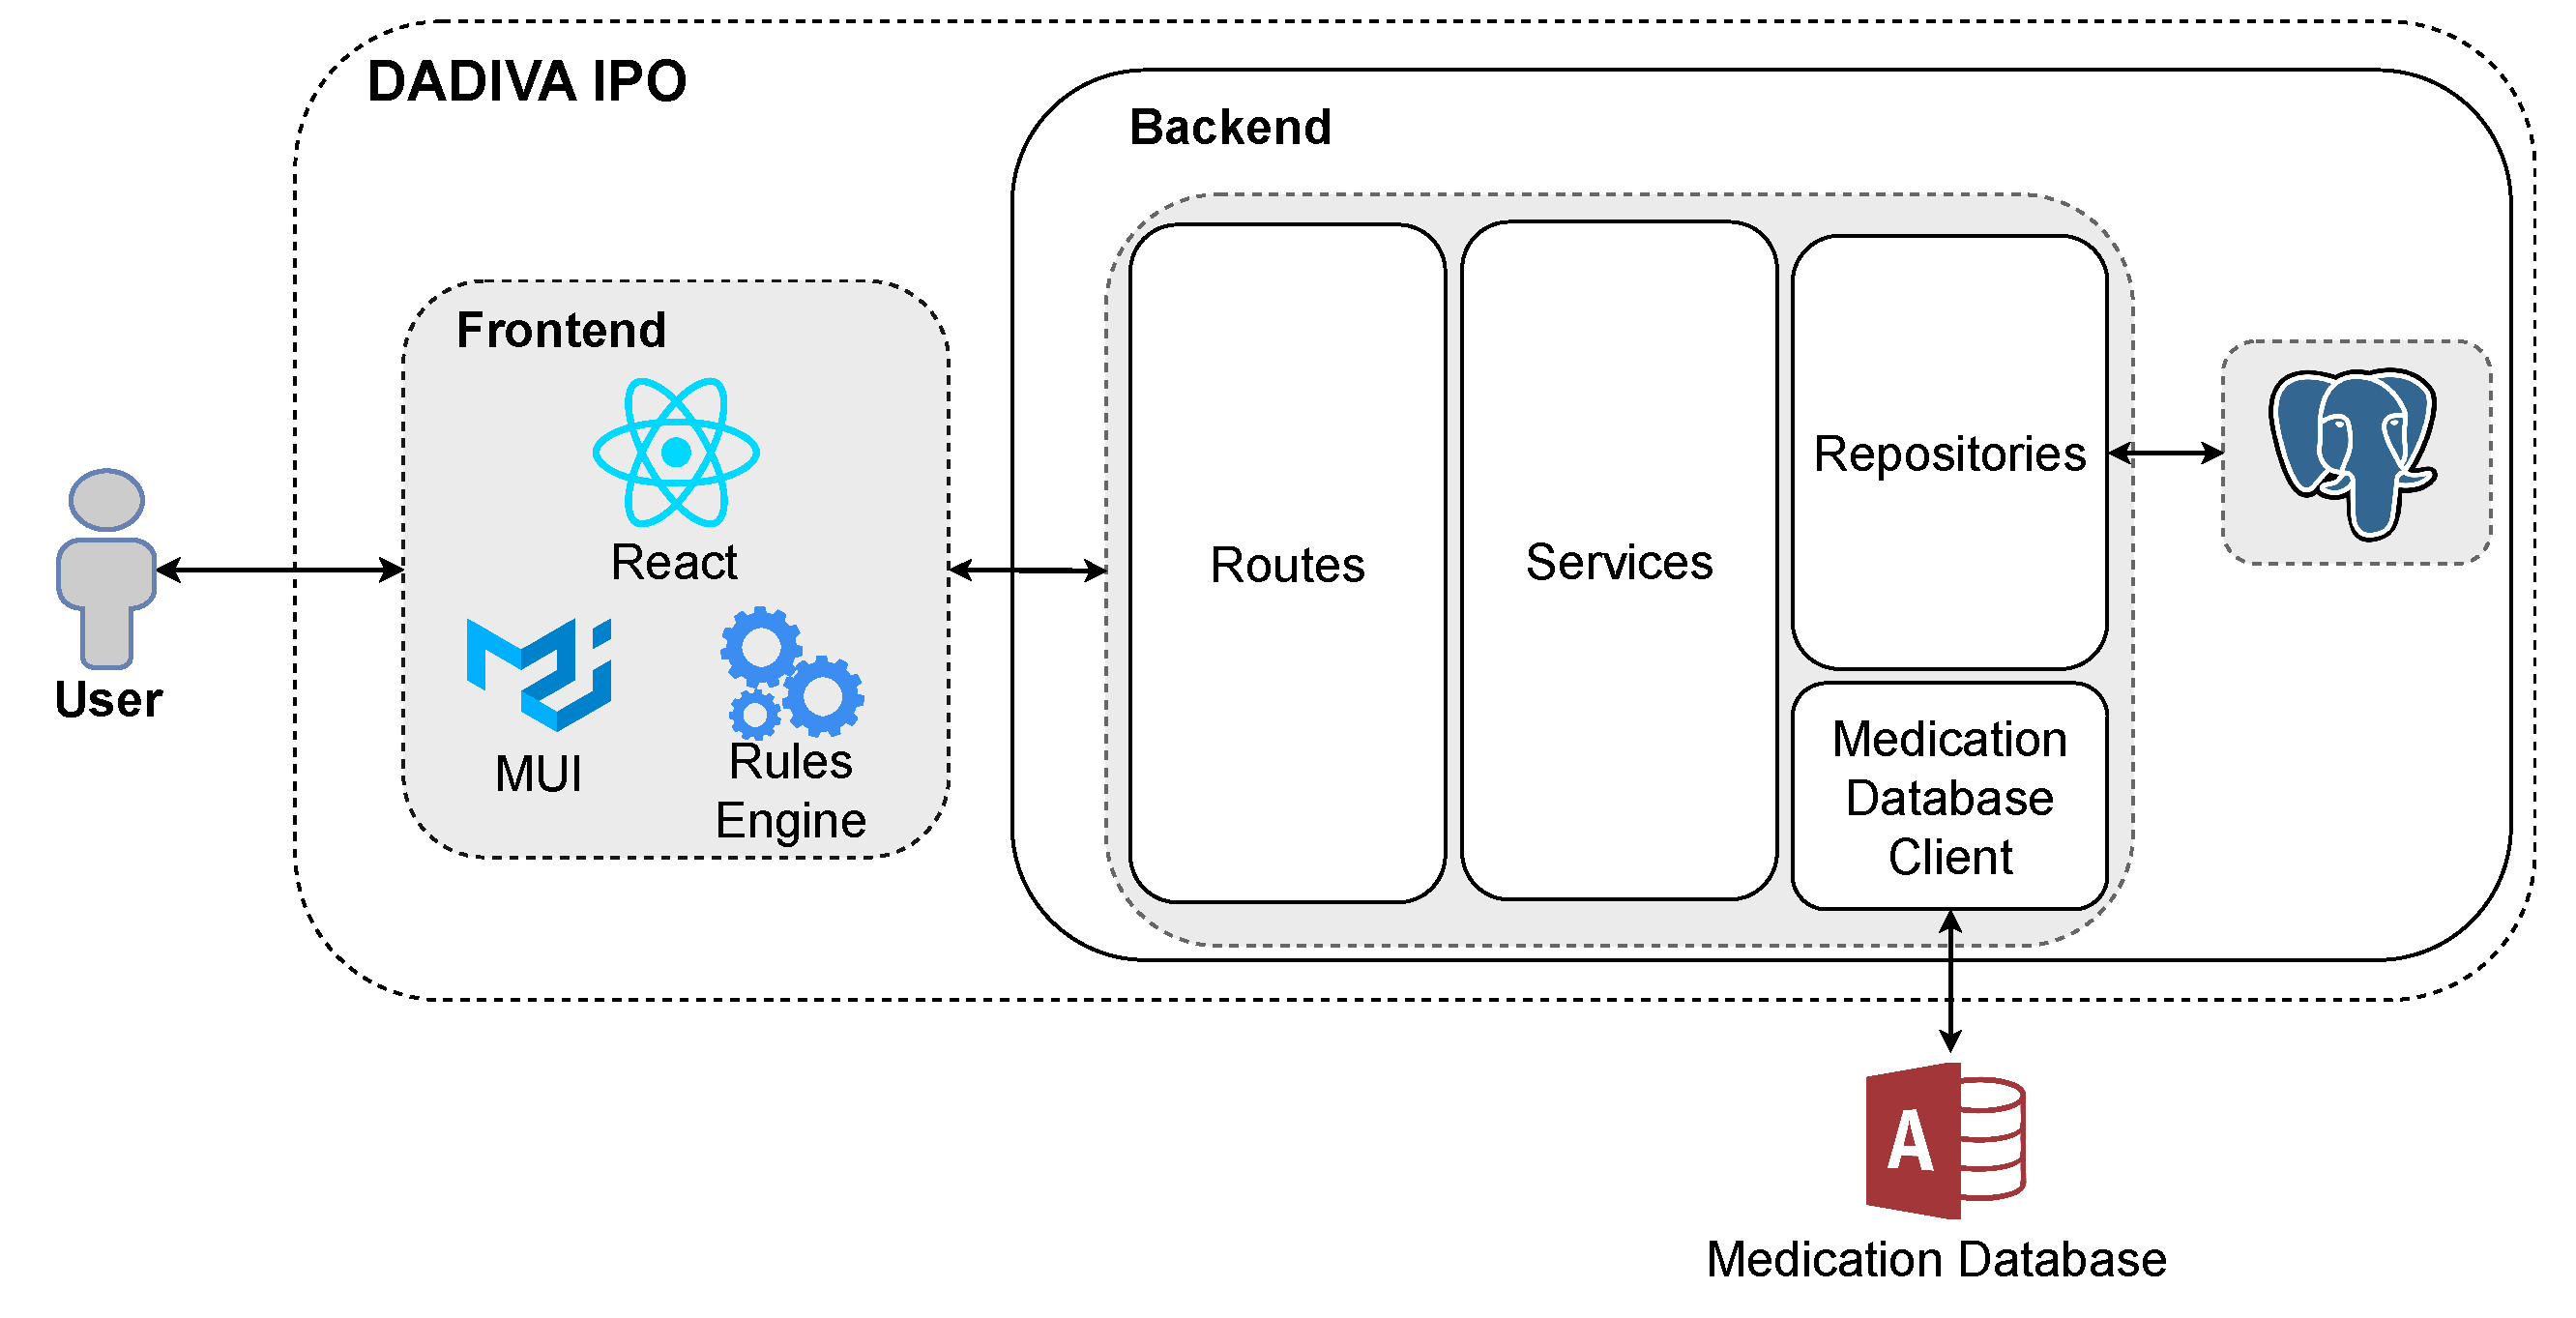
\includegraphics{./figures/Architecture.pdf}}
	\end{center}
	\caption{Application Architecture, gray squares represent containerized components of the solution.}\label{fig:architecture}
\end{figure}


\section{Password Security}\label{sec:security}

Two common password attacks are brute force attacks, and side-channel attacks.

Brute force attacks leverage the high computational power of Graphics Processing Units (GPUs) to paralelize password hashing tasks.

Side-channel attacks try get indirect information leaked during the execution of cryptographic algorithms, ie the time or power it takes for a system to hash a password.

\subsection{Mitigation}

Password hashing is a crucial security measure used to protect stored passwords. Instead of saving passwords in plaintext, which can be easily compromised, passwords are transformed into a hashed format using a hashing algorithm.

The work factor is the number of iterations of the hashing algorithm that are performed for each password. The work factor is typically stored in the hash output. It makes calculating the hash more computationally expensive, which in turn reduces the speed and/or increases the cost for which an attacker can attempt to crack the password hash \cite{owasp_password_storage}, which increases the brute-force attack further.
Choosing a work factor requires a compromise between security and performance, since, if to much computing power is required to hash a password the system becomes targetable to denial of service attacks.

Hashing algorithms that employ constant time operations and parallelism whenever possible help mitigate the risk of side channel attacks, as these factors increases the difficulty to extract information form side-channels.  


\subsection{Argon2id}
Argon2\cite{rfc9106} is a state-of-the-art password hashing algorithm that won the Password Hashing Competition in 2015. It comes in three variants: Argon2d, Argon2i, and Argon2id. Argon2id is a hybrid version that combines the benefits of both Argon2d (which provides resistance against brute-force attacks) and Argon2i (which is designed for side-channel attack resistance), and will be the algorithm used to secure the passwords for our platform.

Argon2id takes in configurable parameter, such as:
\begin{itemize}
	\item \textbf{Memory Cost}: The amount of memory (in kilobytes) used by the algorithm;
	\item \textbf{Time Cost} : The number of iterations the algorithm runs, which affects the computation time;
	\item \textbf{Parallelism} : The number of parallel threads used to process the hash.
\end{itemize}

Since these parameters are configurable it is possible to adjust them throughout the lifetime of an application, for example increase the time cost as the hosting hardware's capacity increases, and decrease it if concurrent accesses increase.

\section{IPO Medication Portal}
\textcolor{red}{
	The IPST medication guideline are organized in a table like manner, in the following column layout:
	\begin{enumerate}
		\item Class/Group of Medication: This column categorizes medications.
		\item Active Substance/Commercial Name: This column lists either the active ingredient or the brand name of the medication.
		\item Criteria: This column specifies if a particular class or group of medications affects eligibility for blood donation, including details such as the duration of ineligibility and other relevant conditions.
	\end{enumerate}
	The terms used in the first column are, from what we can access, similar to the available pharmacotherapeutic classifications. A reliable source of a drug's pharmacotherapeutic classification is a portal provided by Infarmed to it's partner organizations, such as Lisbon's IPO.
	As such, upon a donor's form submission, assuming they were taking some medication, our application would perform requests to said portal, get the appropriate pharmacotherapeutic classification and, by cross-checking the classification with the term used in the first column of the guidelines, return the relevant information.
	However the terms used in the guidelines don't always reflect the available classifications, and, as such, the platform will employ a dictionary that associates the terms used in the guidelines to pharmacotherapeutic classifications. This dictionary will be updatable by the platform's administrators.
	The fact that the IPST guidelines aren't available in a machine readable format persists.
}

\section{Data Models}\label{sec:data_models}

In this chapter we'll elaborate on the various entities that compose our application and their interactions.
The complete entity relationship diagram is present in Appendix \ref{er}.

\subsection{User}

As outlined in section \ref{sec:use_cases}, our application divides users in roles, with each role being able to perform specific actions, as such, the \textbf{User} entity is a supertype, with roles being the overlapping subtypes of user, as a user can occupy multiple roles, as illustrated in Figure \ref{fig:user_entity}.

\begin{figure}[H]
	\begin{center}
		\resizebox{160mm}{!}{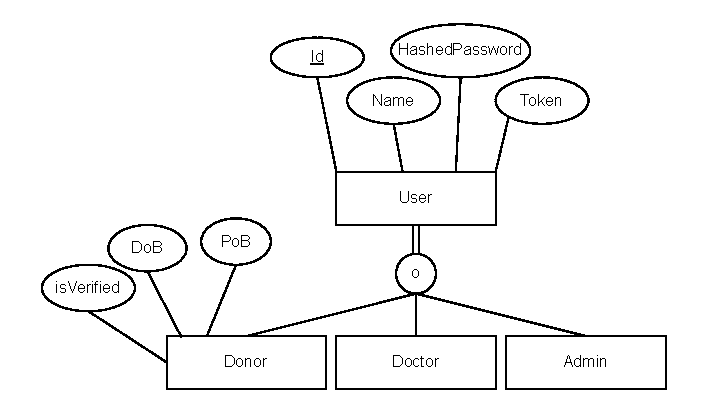
\includegraphics{./figures/User_Entity.pdf}}
	\end{center}
	\caption{User Entity.}\label{fig:user_entity}
\end{figure}

The \textbf{User} supertype contains the attributes that are common to all roles, which are as follows:

\begin{itemize}
	\item Id:A unique identifier which can be a passport or civil identification number;
	\item Name: the user's full name;
	\item HashedPassword: The user's password, stored securely as a hash, more details in section \ref{sec:security};
	\item Token: An authentication token for the user.
\end{itemize}

The \textbf{Donor} subtype contains some specific attributes, which are pertinent to this type, such as:
\begin{itemize}
	\item isVerified: boolean, indicates if donor supplied proof of identity;
	\item DoB: the donor's date of birth;
	\item PoB: the donor's place of birth;
\end{itemize}

\subsubsection{User relationships}

\begin{figure}[H]
	\begin{center}
		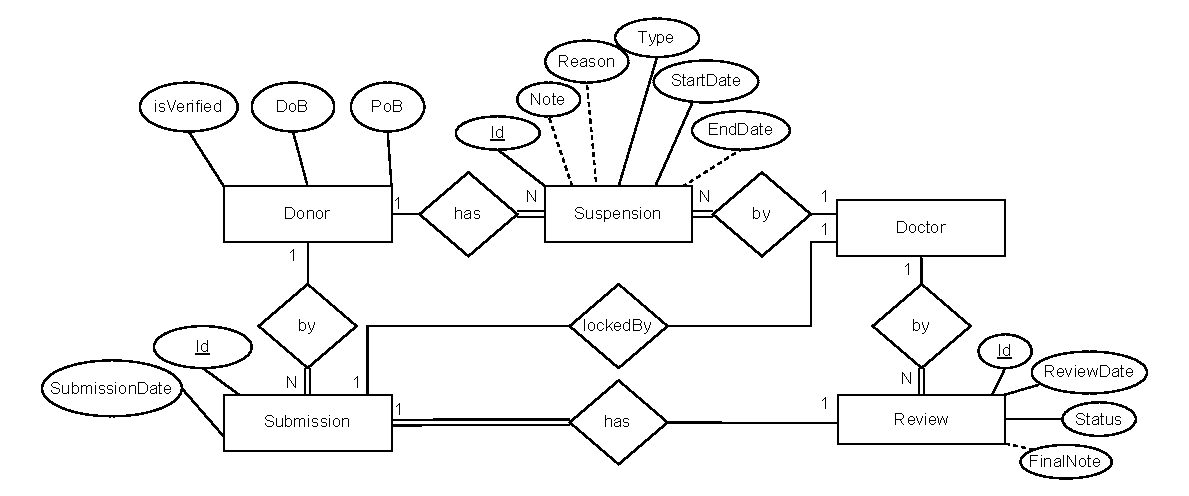
\includegraphics[width=\textwidth,height=\textheight,keepaspectratio]{./figures/User_Interactions.pdf}
	\end{center}
	\caption{User interactions.}\label{fig:user_interactions}
\end{figure}

%As mentioned before, a donor must be verified, this verification is done by an administrator upon first donation when a donor supplies proof of identity.
A \textbf{Donor} can be suspended, ie after a blood donation there's a 2 month waiting period until the next donation, this \textbf{Suspension} is created by a \textbf{Doctor}.
Each \textbf{Donor} can have multiple \textbf{suspensions}, ie multiples waiting periods after donations, and each \textbf{Doctor} can issue multiple \textbf{suspensions}.

The attributes used to characterize a \textbf{Suspension} are as follows:

\begin{itemize}
	\item \textbf{Id}:A unique identifier for the suspension;
	\item \textbf{Type}: Indicates whether the suspension is temporary or permanent;
	\item \textbf{StartDate}: The date when the suspension begins;
	\item \textbf{EndDate}: The date when the suspension ends, optional as permanent suspensions don't have an end date;
	\item \textbf{Reason}: An optional field to specify the reason for the suspension;
	\item \textbf{Note}: An optional note related to the suspension.
\end{itemize}

A \textbf{Donor} performs various pre-donation form \textbf{submissions}, which need to be reviewed by a \textbf{Doctor}, whom can \textbf{review} multiple \textbf{submissions},  with each \textbf{Submission} having a single \textbf{Review}.
The \textbf{Submission} entity's relationships are elaborated on in section \ref{sec:submission}.

A \textbf{Submission} is characterized by the date in which it was performed, \textbf{SubmissionDate}, and a unique identifier.

A review is characterize by the following attribute:
\begin{itemize}
	\item \textbf{Id}:A unique identifier for the Review;
	\item \textbf{ReviewDate}: The date in which the review was performed;
	\item \textbf{Status}: ;
	\item \textbf{FinalNote}: Optional, potential notes;
\end{itemize}





\subsection{Admin}

\begin{figure}[H]
	\begin{center}
		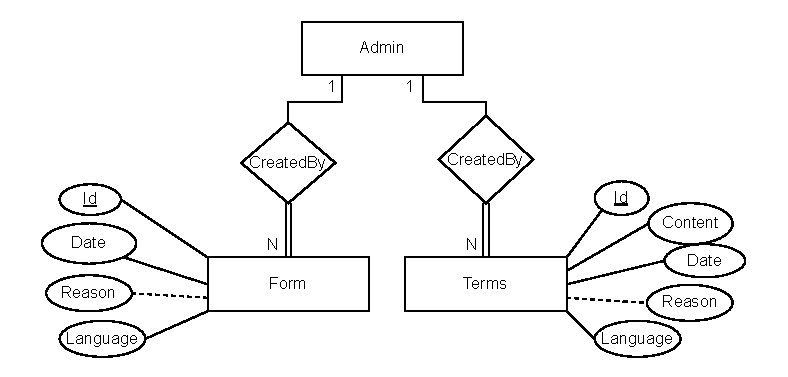
\includegraphics[width=\textwidth,height=\textheight,keepaspectratio]{./figures/Admin_Entity.pdf}
	\end{center}
	\caption{User interactions.}\label{fig:admin_entity}
\end{figure}

An \textbf{Admin} can create multiple pre-donation \textbf{forms} and multiple legal \textbf{terms} for the donation.
The \textbf{Form} entity has more relationships, but to preserve this section's scope that information is omitted but is available in section \ref{sec:form}.

The \textbf{Form} entity is characterized by the following attributes:
\begin{itemize}
	\item \textbf{Id}:A unique identifier for the form;
	\item \textbf{CreatedAt}: The date in which the form was created;
	\item \textbf{Title}: The title of the form, for ease of identification;
	\item \textbf{Language}: The language of the form stored in ISO 639-3;
	\item \textbf{isActive}: Indicates if this form is the one being presented to the donors, only one form can be active at any time for a given language;
\end{itemize}

The \textbf{Terms} entity is characterized by the following attributes:
\begin{itemize}
	\item \textbf{Id}:A unique identifier for the terms;
	\item \textbf{Content}: The actual terms;
	\item \textbf{CreatedAt}: The date in which the terms were created;
	\item \textbf{Title}: The title of the terms, for ease of identification;
	\item \textbf{Language}: The language of the terms;
	\item \textbf{isActive}: Indicates if these terms are being presented to the donors, only one of these entities can be active at any time;
\end{itemize}





\subsection{Form relationships}\label{sec:form}

\begin{figure}[H]
	\begin{center}
		\resizebox{160mm}{!}{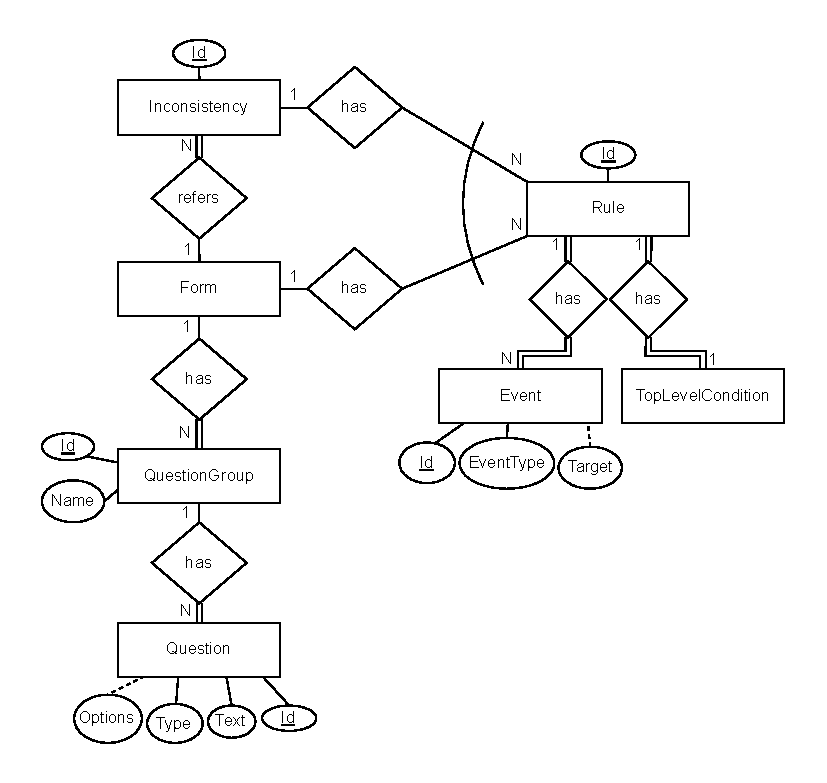
\includegraphics{./figures/Form_Entity.pdf}}
	\end{center}
	\caption{Form Entity.}\label{fig:form_entity}
\end{figure}

A \textbf{Form} is composed of a group of \textbf{questions}, this group represents a theme, and a set of \textbf{rules}, as such it has a one to many relationship with these entities.
For the sake of simplicity a rule can be defined as a logical condition, the \textbf{TopLevelCondition} entity in Figure \ref{fig:form_entity}, that triggers an event when met,ie when a donor answers that he has traveled abroad a subsequent question appears asking to which country, a further explanation of the entities that make up these conditions is presented in section \ref{sec:conditions}.

A \textbf{QuestionGroup} entity has the following attributes:
\begin{itemize}
	\item \textbf{Id}: The group's unique identifier;
	\item \textbf{Name}: The theme of the group, ie travel, health, previous donations, etc;
\end{itemize}

Logically, a \textbf{QuestionGroup} as a one to many relationship with the \textbf{Question} entity.
A \textbf{Question} entity is characterized by the following attributes:
\begin{itemize}
	\item \textbf{Id}: The question's unique identifier;
	\item \textbf{Text}: The actual question;
	\item \textbf{Type}: The type of accepted answer, ie boolean, text, multiple values, etc;
\end{itemize}

An \textbf{Event} entity is characterized by the following attributes:
\begin{itemize}
	\item \textbf{Id}: The event's unique identifier;
	\item \textbf{EventType}: The action the event performs, ie hide/show a question, allow navigation to next group, etc ;
	\item \textbf{Target}: Optional, the target of the action, ie the question to be hidden or displayed;
\end{itemize}

The \textbf{Inconsistency} entity represents a logical fallacy in sets of answers, eg a donor stating the they never traveled outside of Portugal but also stating that they've resided outside of Portugal.
This entity is compromised of a single identifying attribute,Id, and has a one to many relationship with the \textbf{Rule} entity. 


%\subsection{Inconsistency}
%
%\begin{figure}[H]
%	\begin{center}
%		\resizebox{160mm}{!}{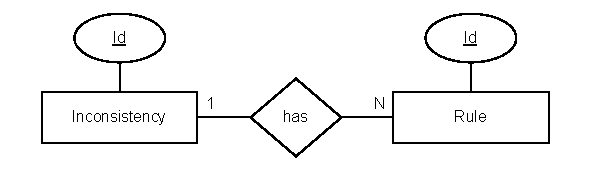
\includegraphics{./figures/Inconsistency_Entity.pdf}}
%	\end{center}
%	\caption{Form Entity.}\label{fig:inconsistency_entity}
%\end{figure}
%
%The inconsistency entity, illustrated in Figure \ref{fig:inconsistency_entity} represents sets of answers that are illogical, ie a donor stating that they've never traveled outside of Portugal but also stating that they've resided outside of Portugal.
%This entity is compromised of a single identifying attribute,Id, and has a one to many relationship with the rule entity,mentioned in subsection \ref{sec:form}.








%\subsection{Rule}\label{sec:rule_entity}
%
%\begin{figure}[H]
%	\begin{center}
%		\resizebox{160mm}{!}{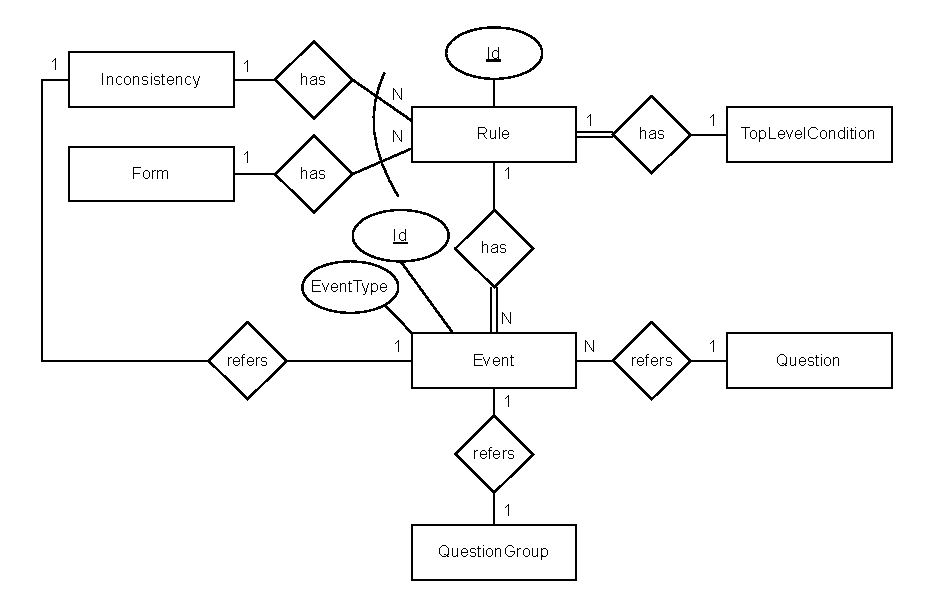
\includegraphics{./figures/Rule_Entity.pdf}}
%	\end{center}
%	\caption{Form Entity.}\label{fig:rule_entity}
%\end{figure}
%
%The rule entity, illustrated in Figure \ref{fig:rule_entity}, has a single identifying attribute, Id, and  can be a part of a form or an inconsistency, as mentioned before.
%It has a one to one relationship with the top level condition entity, which is further elaborated in subsection \ref{conditions}, but, for now, can simply be described as the logical premises of the rule.
%
%If the logical premises are met one or more events might be triggered, hence the event entity and the rule entity have a one to many relationship.
%
%The event entity has the following attributes:
%\begin{itemize}
%	\item Id: The event's unique identifier;
%	\item EventType: The consequence of this event, ie show a question, enable the next question group, or point out inconsistent responses;
%\end{itemize}
%
%As described by the EventType attribute, and event entity can reference a question, a question group or an inconsistency.

\subsection{Conditions}\label{sec:conditions}

\begin{figure}[H]
	\begin{center}
		\resizebox{160mm}{!}{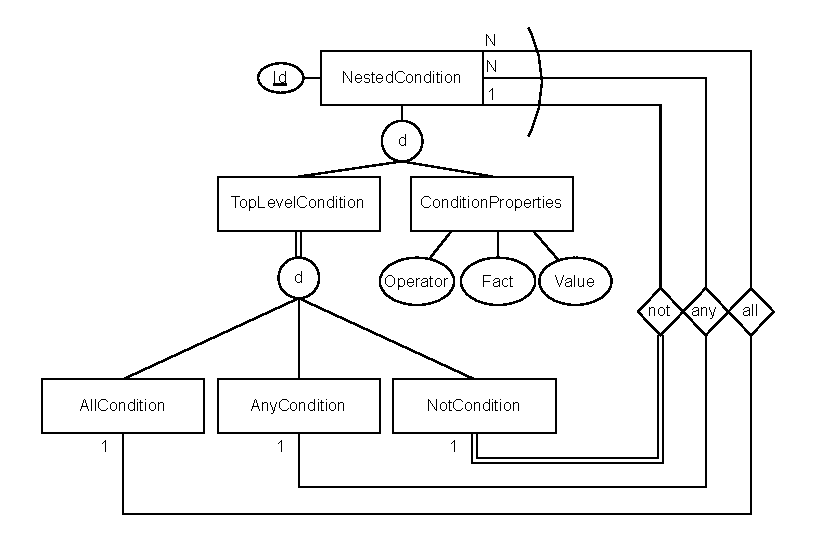
\includegraphics{./figures/Condition_Entity.pdf}}
	\end{center}
	\caption{Condition Entity.}\label{fig:condition_entity}
\end{figure}

The entities and relationships mentioned in this section reflect the types belonging to the \textbf{JSON-Rules-Engine}.
The  \textbf{NestedCondition} entity is a supertype of the \textbf{TopLevelCondition} entity and the \textbf{ConditionProperties} entity.
As the \textbf{TopLevelCondition} entity is a supertype of the \textbf{AllCondition}, \textbf{AnyCondition} a \textbf{NotCondition} entities, it can be seen as a representation of logical operators. As illustrated in Figure \ref{fig:condition_entity}, the \textbf{AllCondition} and \textbf{AnyCondition} entities have a one to many relationship with the \textbf{NestedCondition}, while the \textbf{NotCondition} as a one to one relationship, this means the \textbf{all} and \textbf{any} conditions can have multiple conditions nested inside them while the \textbf{not} condition can have a single condition nested inside it, which allows for the creation of complex boolean expressions.

The \textbf{ConditionProperties} entity represents a logical evaluation and has the following attributes:
\begin{itemize}
	\item \textbf{Operator}: The logical operator of the evaluation, ie equal, less than, greater than, etc;
	\item \textbf{Fact}: The id of the question being evaluated;
	\item \textbf{Value}: The expected value of the question being referenced.
\end{itemize}





\subsection{Submission}\label{sec:submission}

\begin{figure}[H]
	\begin{center}
		\resizebox{160mm}{!}{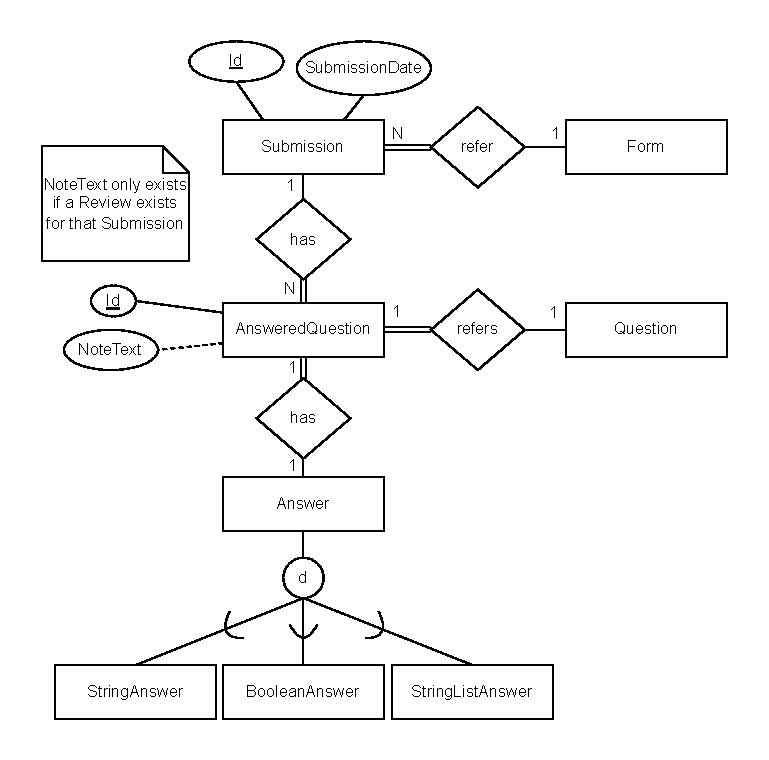
\includegraphics{./figures/Submission_Entity.pdf}}
	\end{center}
	\caption{Submission Entity.}\label{fig:submission_entity}
\end{figure}

As illustrated in Figure \ref{fig:submission_entity}, the \textbf{Submission} entity as a relationship with the \textbf{Form} entity, since a given submission pertains to a certain version of the form which changes overtime, and with the \textbf{AnsweredQuestion} entity,this entity has a \textbf{NoteText} attribute, which is optional, and represents a doctor note about the answer provided and a relationship with the \textbf{Question} entity, since every answer must refer to a question in the form.
The \textbf{AnsweredQuestion} entity also has a relationship with the \textbf{Answer} entity which is a supertype representing the possible values for the form's answers.



\subsection{Change Log}

\begin{figure}[H]
	\begin{center}
		\resizebox{160mm}{!}{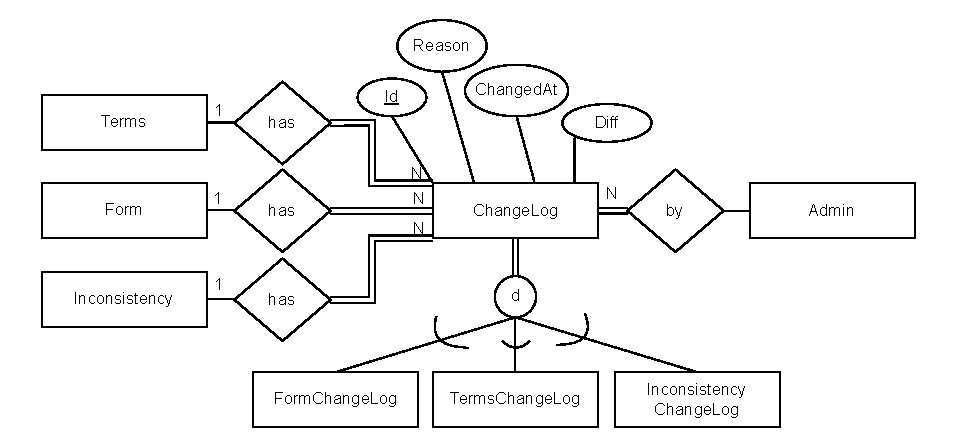
\includegraphics{./figures/ChangeLog_Entity.pdf}}
	\end{center}
	\caption{ChangeLog Entity.}\label{fig:changelog_entity}
\end{figure}

To enforce admin accountability for \textbf{term}, \textbf{form} and \textbf{inconsistency} changes the \textbf{ChangeLog} entity was created and is illustrated in Figure \ref{fig:changelog_entity}.

This entity has relationships with all the entities that are subjected to change and with the \textbf{Admin} entity that performed the changes.

The \textbf{ChangeLog} entity serves as a supertype of the possible changes to the system, and it as the following attributes:
\begin{itemize}
	\item \textbf{Id}: The ChangeLog's unique identifier;
	\item \textbf{Reason}: Optional, reason for the change;
	\item \textbf{ChangedAt}: The date the change was performed;
	\item \textbf{Diff}: What was changed;
\end{itemize}






\subsection{Manual Information}

\begin{figure}[H]
	\begin{center}
		\resizebox{160mm}{!}{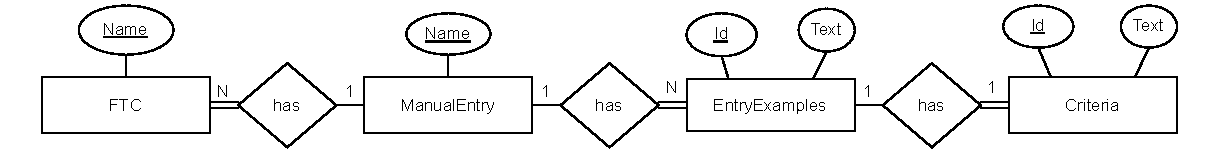
\includegraphics{./figures/Manual_Entity.pdf}}
	\end{center}
	\caption{Manual Entity.}\label{fig:manual_entity}
\end{figure}

To allow doctors to search for medication interactions with blood donations and to perform the risk vector analysis we created the \textbf{FTC} entity which is the pharmaco-therapeutic classification of the medication.
This entity has an identifying \textbf{Name} attribute, which is the name for this group of medications, e.g. analgesics and antipyretics, non steroidal anti inflammatories, etc.

The \textbf{ManualEntry} entity has an identifying \textbf{Name} attribute, which is the name used to group medications in the manual.

The \textbf{FTC} and \textbf{ManualEntry} entities have a many to one relationship as the names used in the manual might refer to more than one classification, and will possibly not have a match with any \textbf{FTC}.

The \textbf{EntryExamples} entity represents the examples presented in the manual for each entry, ie in the 2022 manual the analgesics entry contains two examples "Paracetamol, Ben U Ron, Tramadol..." and "Opioid Analgesics", so this entity has a many to one relationship with the \textbf{ManualEntry} entity and an attribute \textbf{Text}, with the examples.

Finally the \textbf{Criteria} entity which refers to whether a donor is able to donate blood or should be suspended, and whether that suspension is temporary or permanent if he's taken this medication. This entity as a one to one relationship with \textbf{EntryExamples} entity, as the evaluation of blood donation capabilities is dependent on these examples, since different medications within the same classification can lead to distinct outcomes.














\section{Backend Application}

The backend application can be abstracted into 4 layers:
\begin{itemize}
	\item Routes: responsible for receiving the http request and calling the correct service;
	\item Services: contains the services that manage the business logic of the application;
	\item Medication Database Client: responsible for requesting information to IPO's medication database;
	\item Repositories: contains the repository layer of the application;
\end{itemize}

With each one of these layers being divided by groups of functions that deal with a certain data model, such:
\begin{itemize}
	\item form;
	\item manual;
	\item medications;
	\item users;
\end{itemize}

\subsection{Error Handling}

When an error occurs in the backend, it is crucial not to expose any sensitive information, such as the exception thrown. Exposing raw exceptions can lead to security vulnerabilities and may leak implementation details that could be exploited by malicious actors. To handle errors safely and effectively, we will utilize a \textbf{Result} class.

The \textbf{Result} class can represent two states: \textbf{Success} or \textbf{Problem}.
\begin{itemize}
	\item \textbf{Success}: This state indicates that the request was processed successfully. It encapsulates the result of the operation, ensuring that the expected outcome is communicated clearly to the client.
	\item \textbf{Problem}: This state is defined in accordance with RFC 7807\cite{rfc7807}. The \textbf{Problem} class provides a standardized way to convey error information. It ensures that detailed error information is supplied without exposing sensitive data. By following the RFC 7807 specification, the Problem class includes the following fields:
	\begin{itemize}
		\item \textbf{'type'}: A URI reference that identifies the problem type. This URI is intended to provide human-readable documentation for the specific problem encountered.
		\item \textbf{'title'}: A short, human-readable summary of the problem type. This remains consistent across occurrences of the same problem type, making it easier for developers to recognize recurring issues.
		\item \textbf{'status'}:  The HTTP status code generated by the origin server for this particular occurrence of the problem. This aligns with standard HTTP status codes, facilitating easy interpretation by both humans and machines.
		\item \textbf{'details'}: A human-readable explanation specific to this instance of the problem. It provides more context and helps in understanding the error without revealing sensitive information.
	\end{itemize}
\end{itemize}

The \textbf{Problem} class's standardized format ensures that error information is conveyed consistently, which enhances both the readability for humans and the parsability for machines. This consistency is vital for effective debugging, logging, and automated error handling.

When possible the 'title' and 'details' fields should follow some guideline to ensure security, such as owasp's recommendation for authentication error responses \cite{owasp_authentication}, which states that "using any of the authentication mechanisms (login, password reset, or password recovery), an application must respond with a generic error message regardless of whether:The user ID or password was incorrect.The account does not exist.The account is locked or disabled."

An example of the flow for GET form resource request is presented in Figure ~\ref{fig:getForm_Sequence_Diagram}

\begin{figure}[H]
	\begin{center}
		\resizebox{160mm}{!}{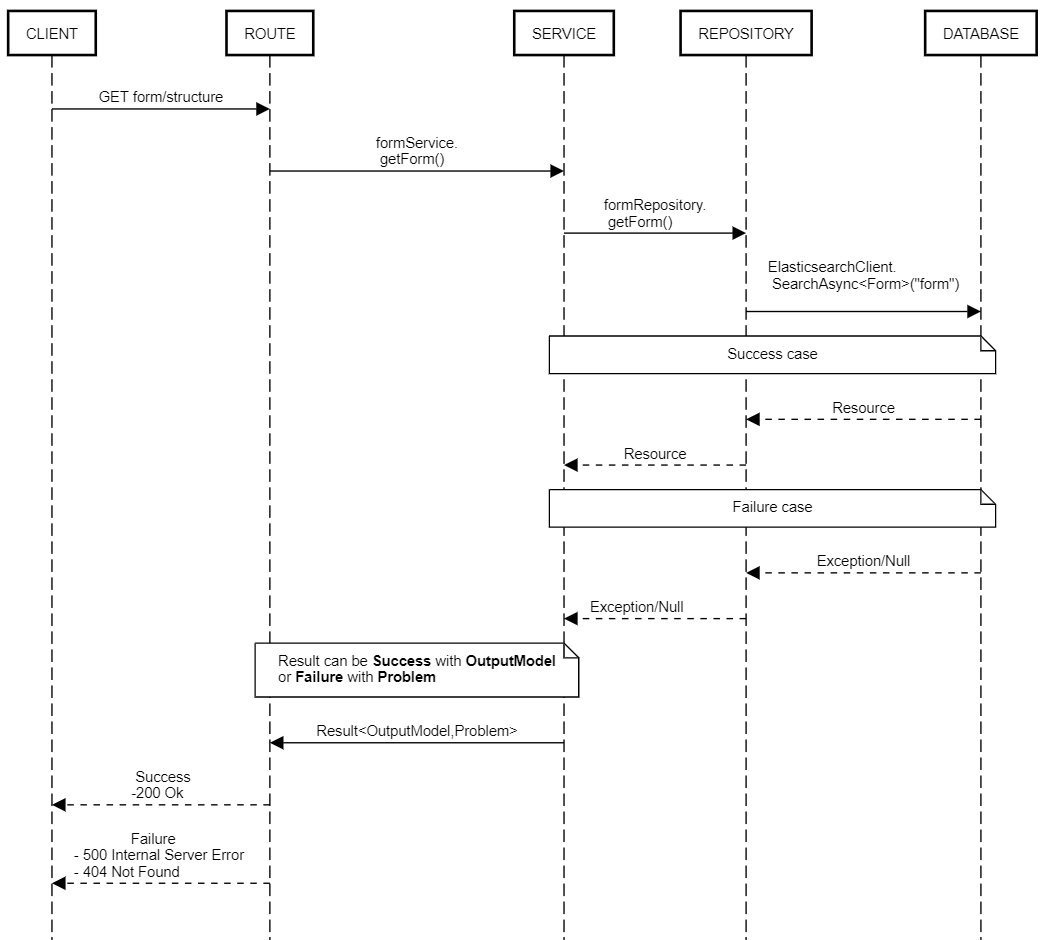
\includegraphics{./figures/getForm_Sequence_Diagram.png}}
	\end{center}
	\caption{Get Form Sequence Diagram.}\label{fig:getForm_Sequence_Diagram}
\end{figure}

%The backend handles HTTP requests directed to specific endpoints. The route associated with each endpoint converts the request body into an appropriate model, if necessary, and then calls the corresponding service, passing along the model. The service validates the model, converts it into a domain object, and calls the relevant repository. Using an ElasticClient, the repository stores the object in the ElasticSearch database. The appropriate response is then propagated back up, as illustrated in Figure ~\ref{fig:backendLayers}.
%
%\begin{figure}[H]
%	\begin{center}
%		\resizebox{100mm}{!}{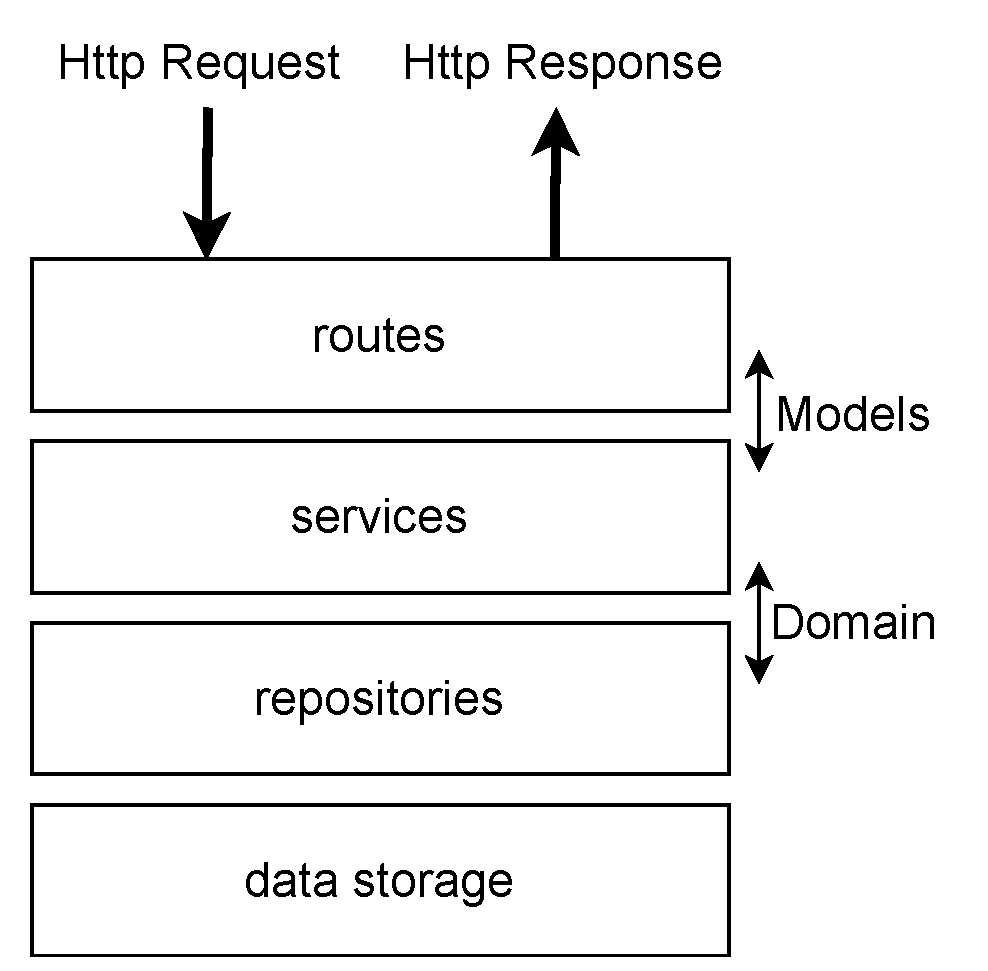
\includegraphics{./figures/backendLayers.pdf}}
%	\end{center}
%	\caption{Backend layers.}\label{fig:backendLayers}
%\end{figure}




%\section{Form Data Model and Inconsistencies Data Model}

%The first approach to solve the dynamic form challenge was to use a data structure formed by pairs of main questions and sub-questions, example presented in Figure ~\ref{fig:old_form}, where a main question can only be answered with boolean values, and one of those values triggers the display of a sub-question which has a certain type of response, such as boolean, dropdown for known multiple answers, and text, to accept user text input.

%\begin{figure}[hbt!]
%	\begin{center}
%		\resizebox{150mm}{!}{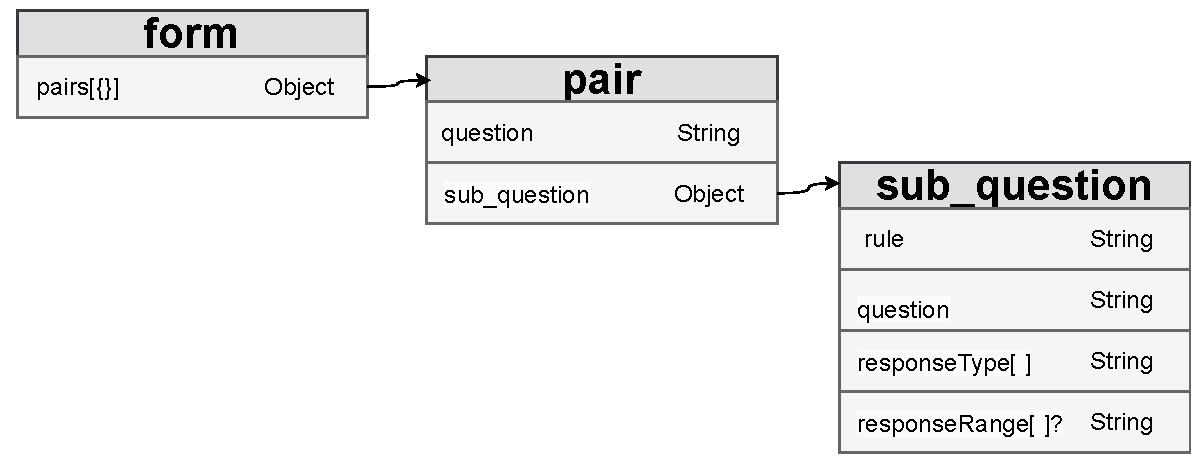
\includegraphics{./figures/oldForm.pdf}}
%	\end{center}
%	\caption{First Form Data Structure.}\label{fig:old_form}
%\end{figure}
%
%This approach has several drawbacks. Firstly, it prevents the suppression of further questions, which contradicts the goal of creating a flexible and adaptable solution. Additionally, it conflates questions and rules within sub-questions, leading to a lack of clarity and potential confusion in implementation.
%
%Upon further discussion we settled on using a more complex data structure , exemplified in Figure ~\ref{fig:new_form}, composed by a list of questions and a list of rules.
%
%Each question has an id, the text that composes it, the type of response (boolean, text and dropdown) and can have options that lists all the possibles values for a multiple(dropdown) response.
%
%Each rule has conditions, which can be "any","all" or "not", so that, when any, all or none of the conditions are met an event is triggered.
%Each condition type will have a fact, an operator and a value. In essence, when a question, which is identified by the fact field via it's id, is answered a condition can true or false depending on the logical operator used, ie equal or notEqual, and the value of the answer. If the condition is true an event is triggered, this event can be to show or hide a subsequent question, this targeted question is identified via the id, supplied in the params field.
%
%This model, specifically the rules field, was chosen as it is part of the JSON-Rules-Engine specification, which is presented in more detail in Chapter ~\ref{cap:technologies} and is easily stored and retrieved in a ElasticSearch database.
%
%\begin{figure}[htbp]
%	\begin{center}
%		{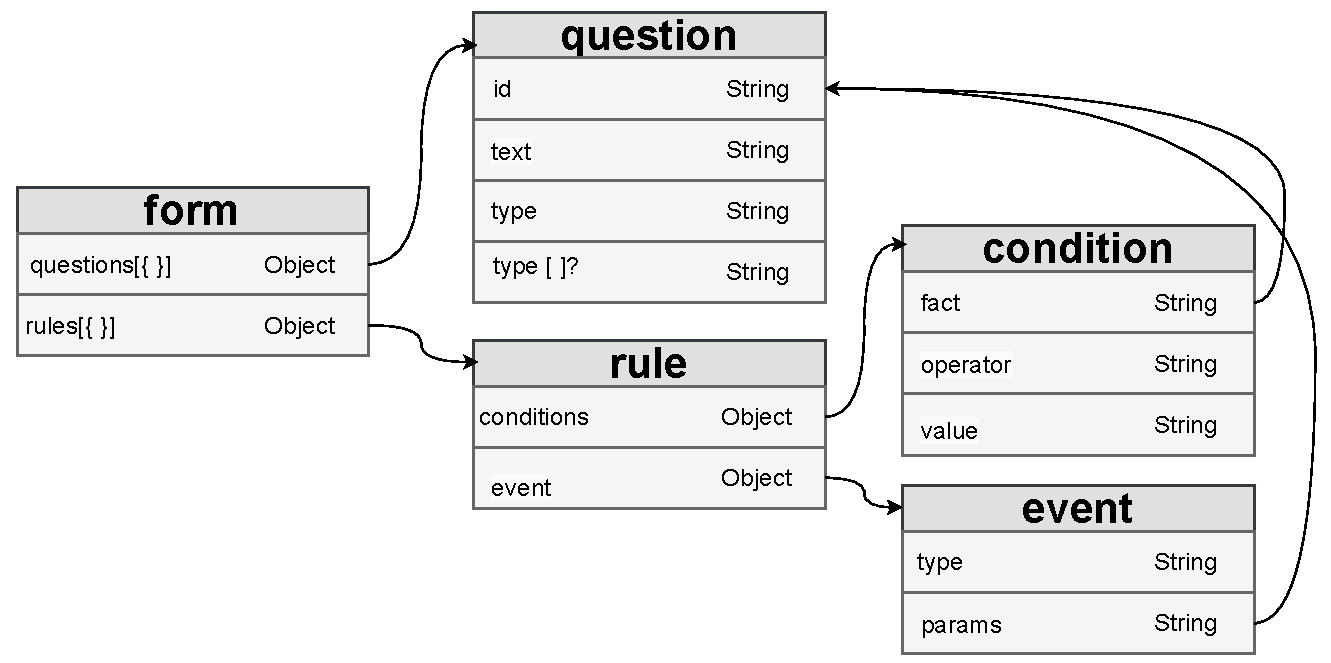
\includegraphics[width=\textwidth,height=\textheight,keepaspectratio]{./figures/newForm.pdf}}
%	\end{center}
%	\caption{Final Form Data Structure.}\label{fig:new_form}
%\end{figure}
%\FloatBarrier
%
%The inconsistencies data model is compromised of rules, and describes answer combinations that are logical fallacies, ie a donor answering that they're healthy in one question and that they have a chronic disease in another question.
%
%\section{Submission Data Model}
%
%The submission data structure represents and answered form, has such it contains a list of answered questions, each answered question is composed by the question id and the answer, as referenced in Figure ~\ref{fig:submission_data_model}.
%
%\begin{figure}[hbt!]
%	\begin{center}
%		\resizebox{150mm}{!}{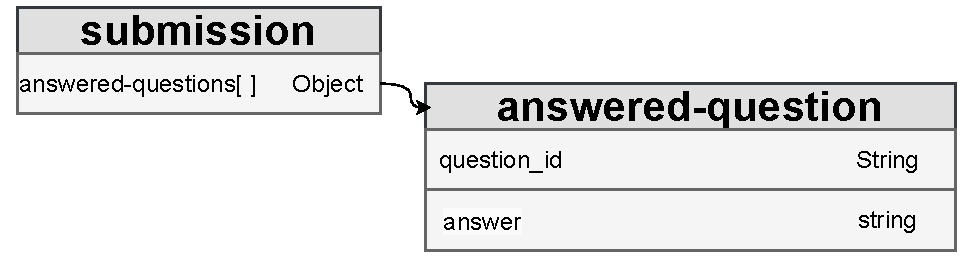
\includegraphics{./figures/Submission_Data_Model.pdf}}
%	\end{center}
%	\caption{Submission Data Structure.}\label{fig:submission_data_model}
%\end{figure}
%
%
%\section{User Data Model}
%
%The user data structure is composed on an unique identifier, the nic, and the user hashed password, as referenced in Figure ~\ref{fig:user_data_model}.
%
%\begin{figure}[hbt!]
%	\begin{center}
%		\resizebox{150mm}{!}{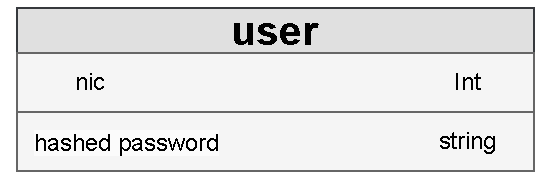
\includegraphics{./figures/User_Data_Structure.pdf}}
%	\end{center}
%	\caption{User Data Structure.}\label{fig:user_data_model}
%\end{figure}

%%secalhar é mais adequado na descrição do problema




\section{Frontend Application}\label{architecture_frontend}

The frontend application is a web-based interface designed to facilitate seamless interaction between users and the backend system. It features a user-friendly and intuitive interface, catering to different types of users with specific functionalities:

\begin{itemize}
	\item Donor Users: Can fill out the current donation form;
	\item Doctor Users: Can search for pathology and medication interactions with blood donation and request form answers for specific users;
	\item Administrator Users: Can customize the current form, update pathology and medication interaction information, update the inconsistencies and manage users.
\end{itemize}

The application is organized into multiple pages and components, each serving distinct purposes. It includes a service layer responsible for communicating with the backend application through the REST API.

During planning some mockups where created of the final result for some pages, the login page is presented in Figure ~\ref{fig:login}, the form pages are presented in Figures ~\ref{fig:form},~\ref{fig:form_no} and ~\ref{fig:form_yes}, the backoffice page is presented in Figure ~\ref{fig:backoffice}.

\begin{figure}[H]
	\begin{center}
		\resizebox{160mm}{!}{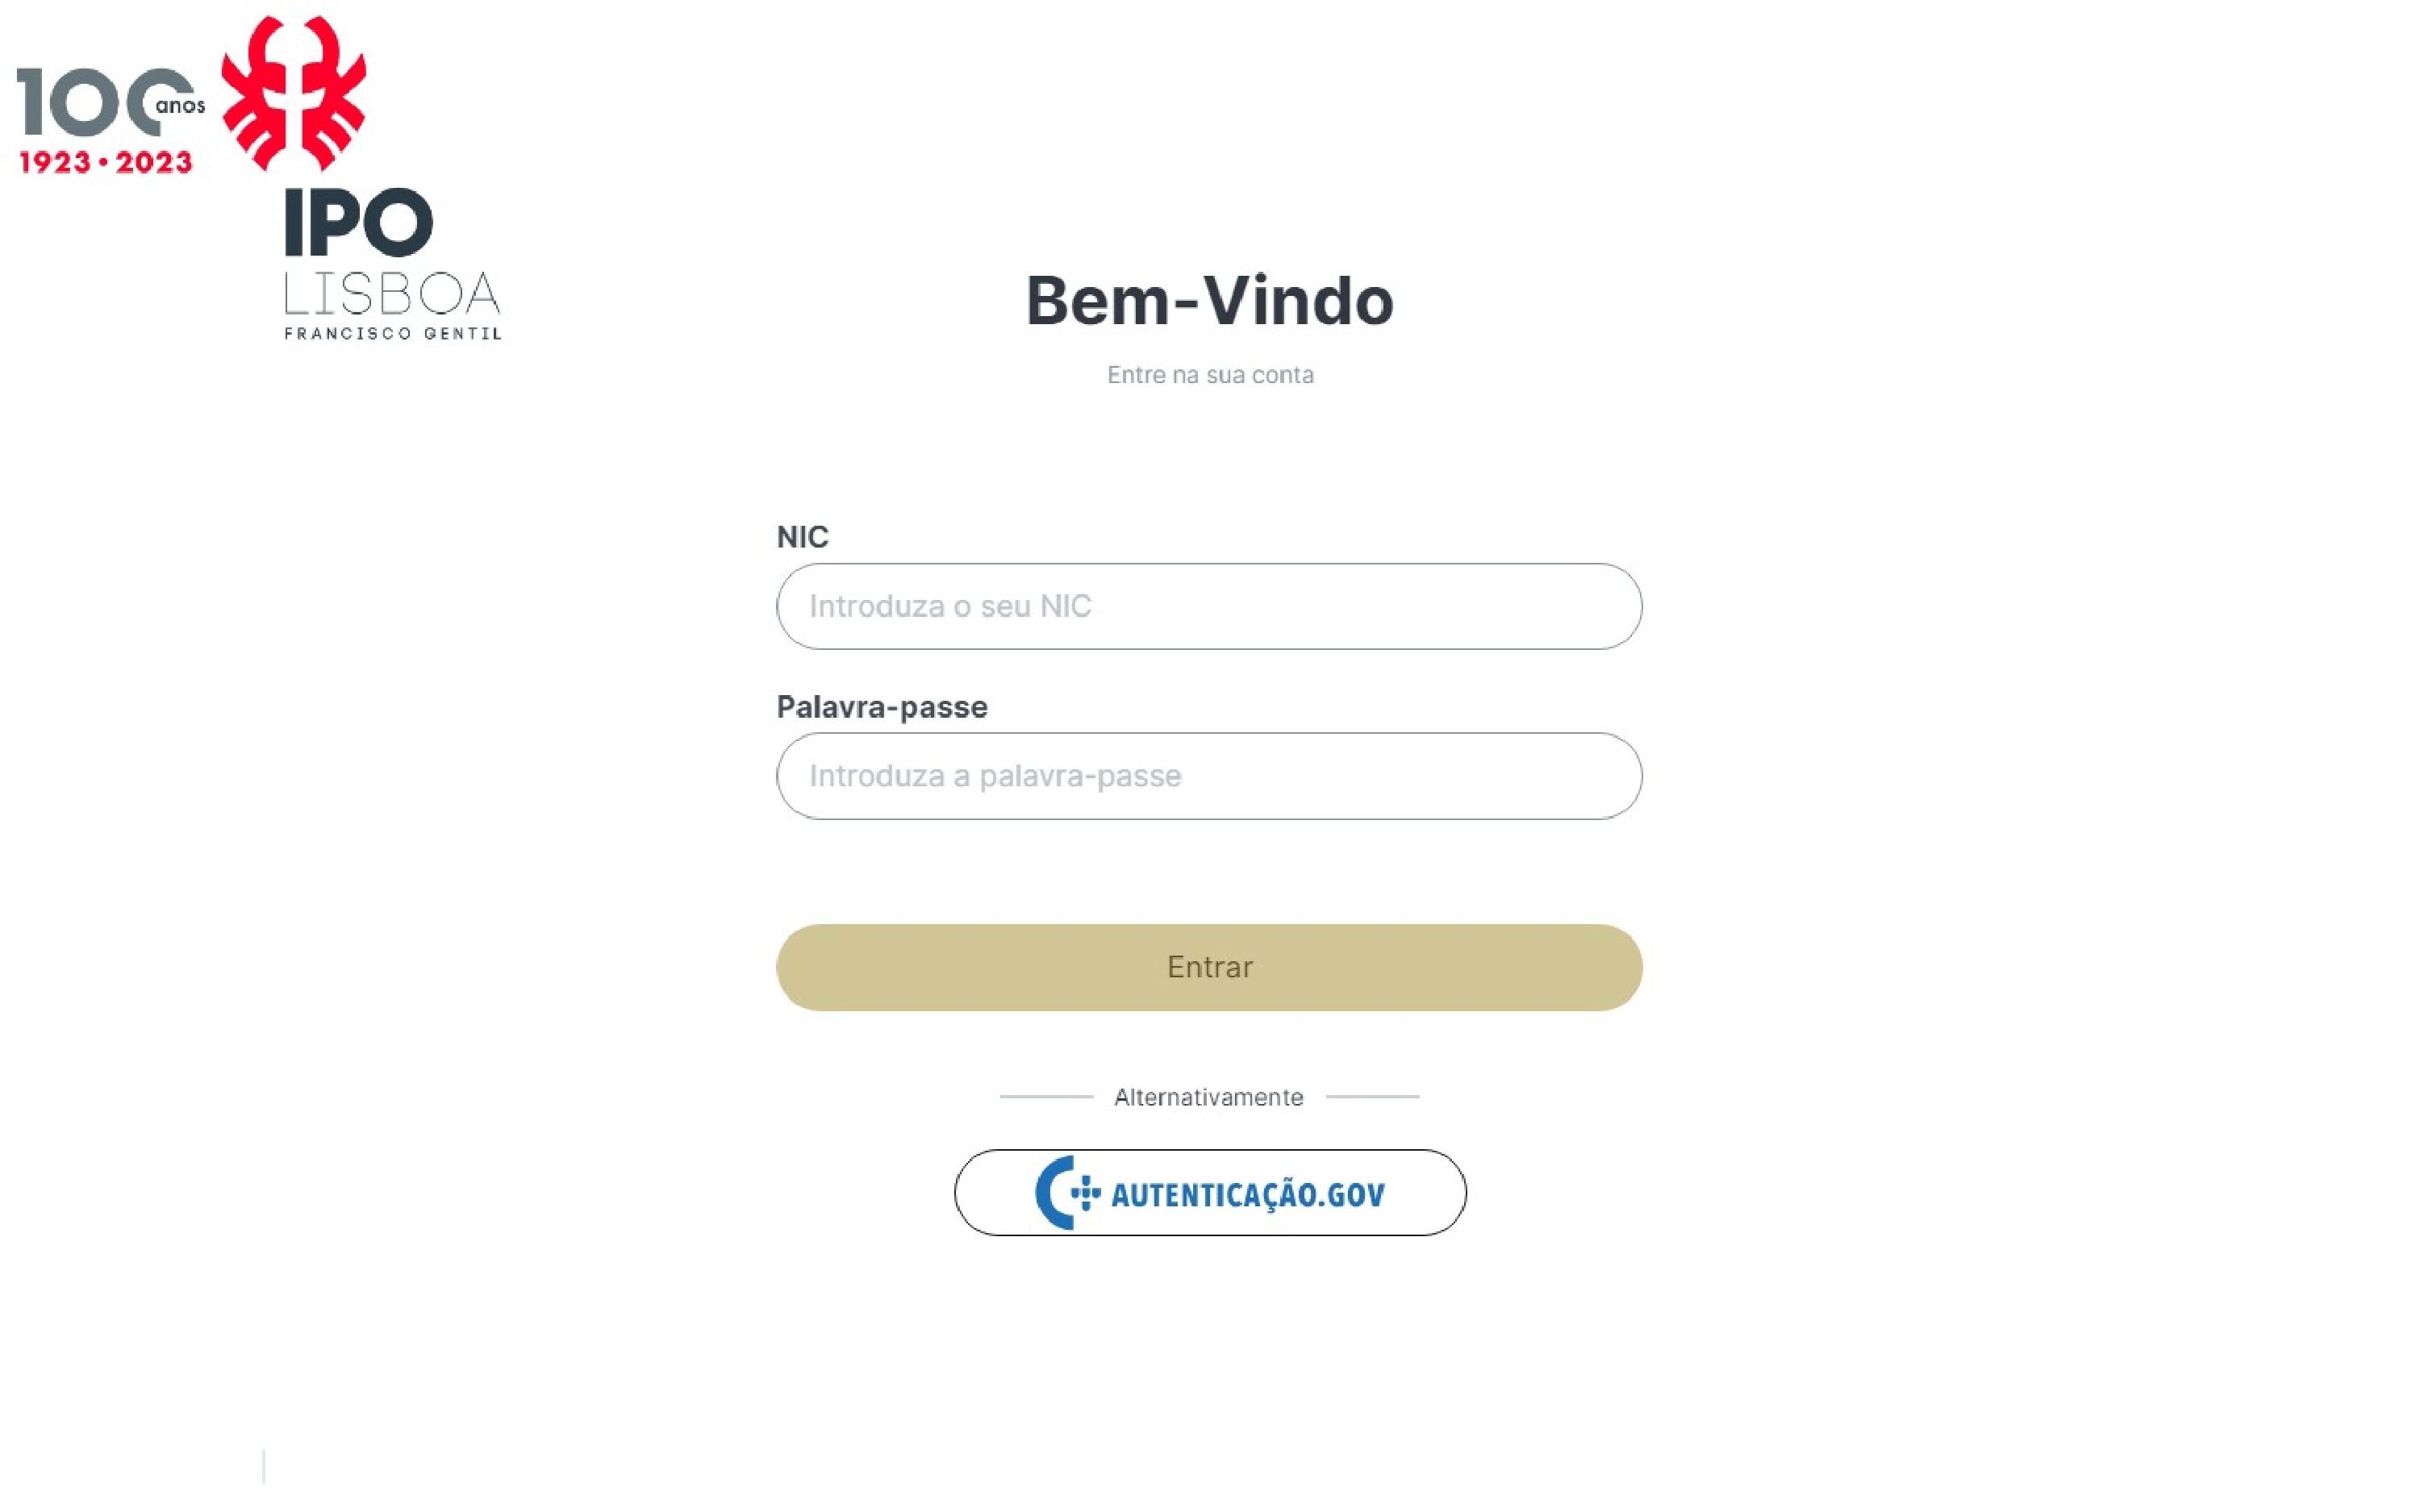
\includegraphics{./figures/Login.pdf}}
	\end{center}
	\caption{Login Page Mock.}\label{fig:login}
\end{figure}

\begin{figure}[H]
	\begin{center}
		\resizebox{160mm}{!}{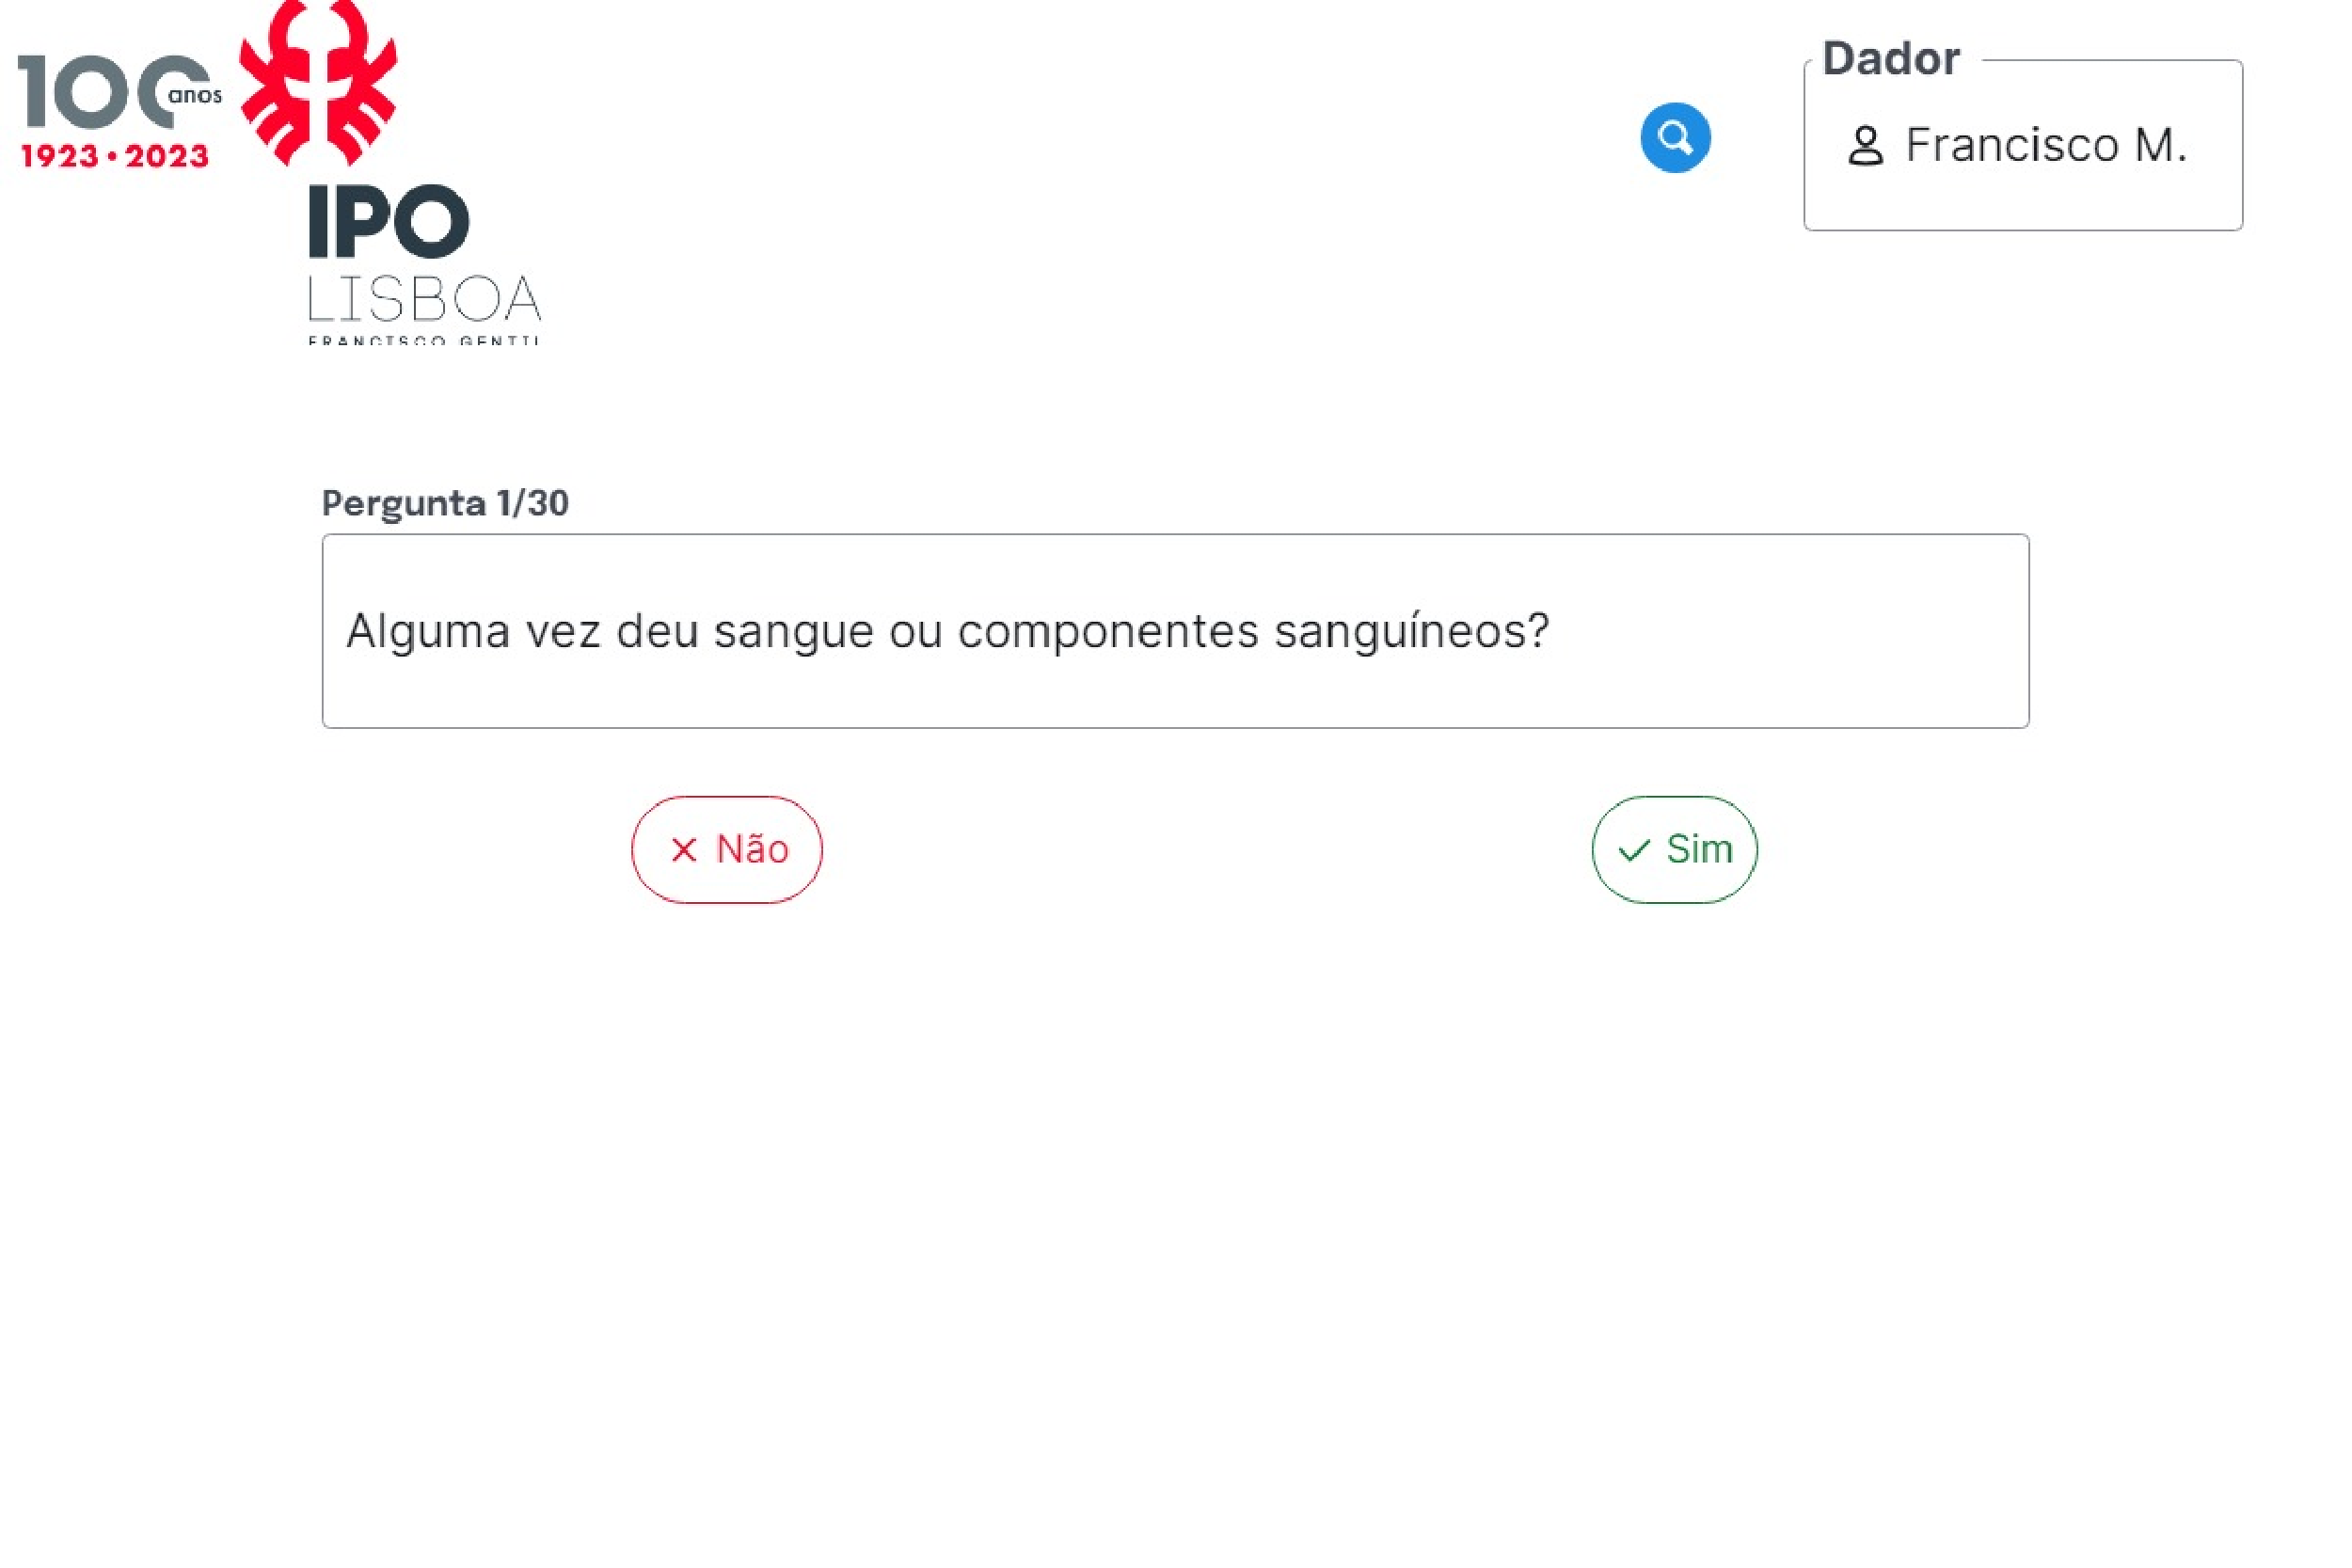
\includegraphics{./figures/Form.pdf}}
	\end{center}
	\caption{Form Page Mock.}\label{fig:form}
\end{figure}

\begin{figure}[H]
	\begin{center}
		\resizebox{160mm}{!}{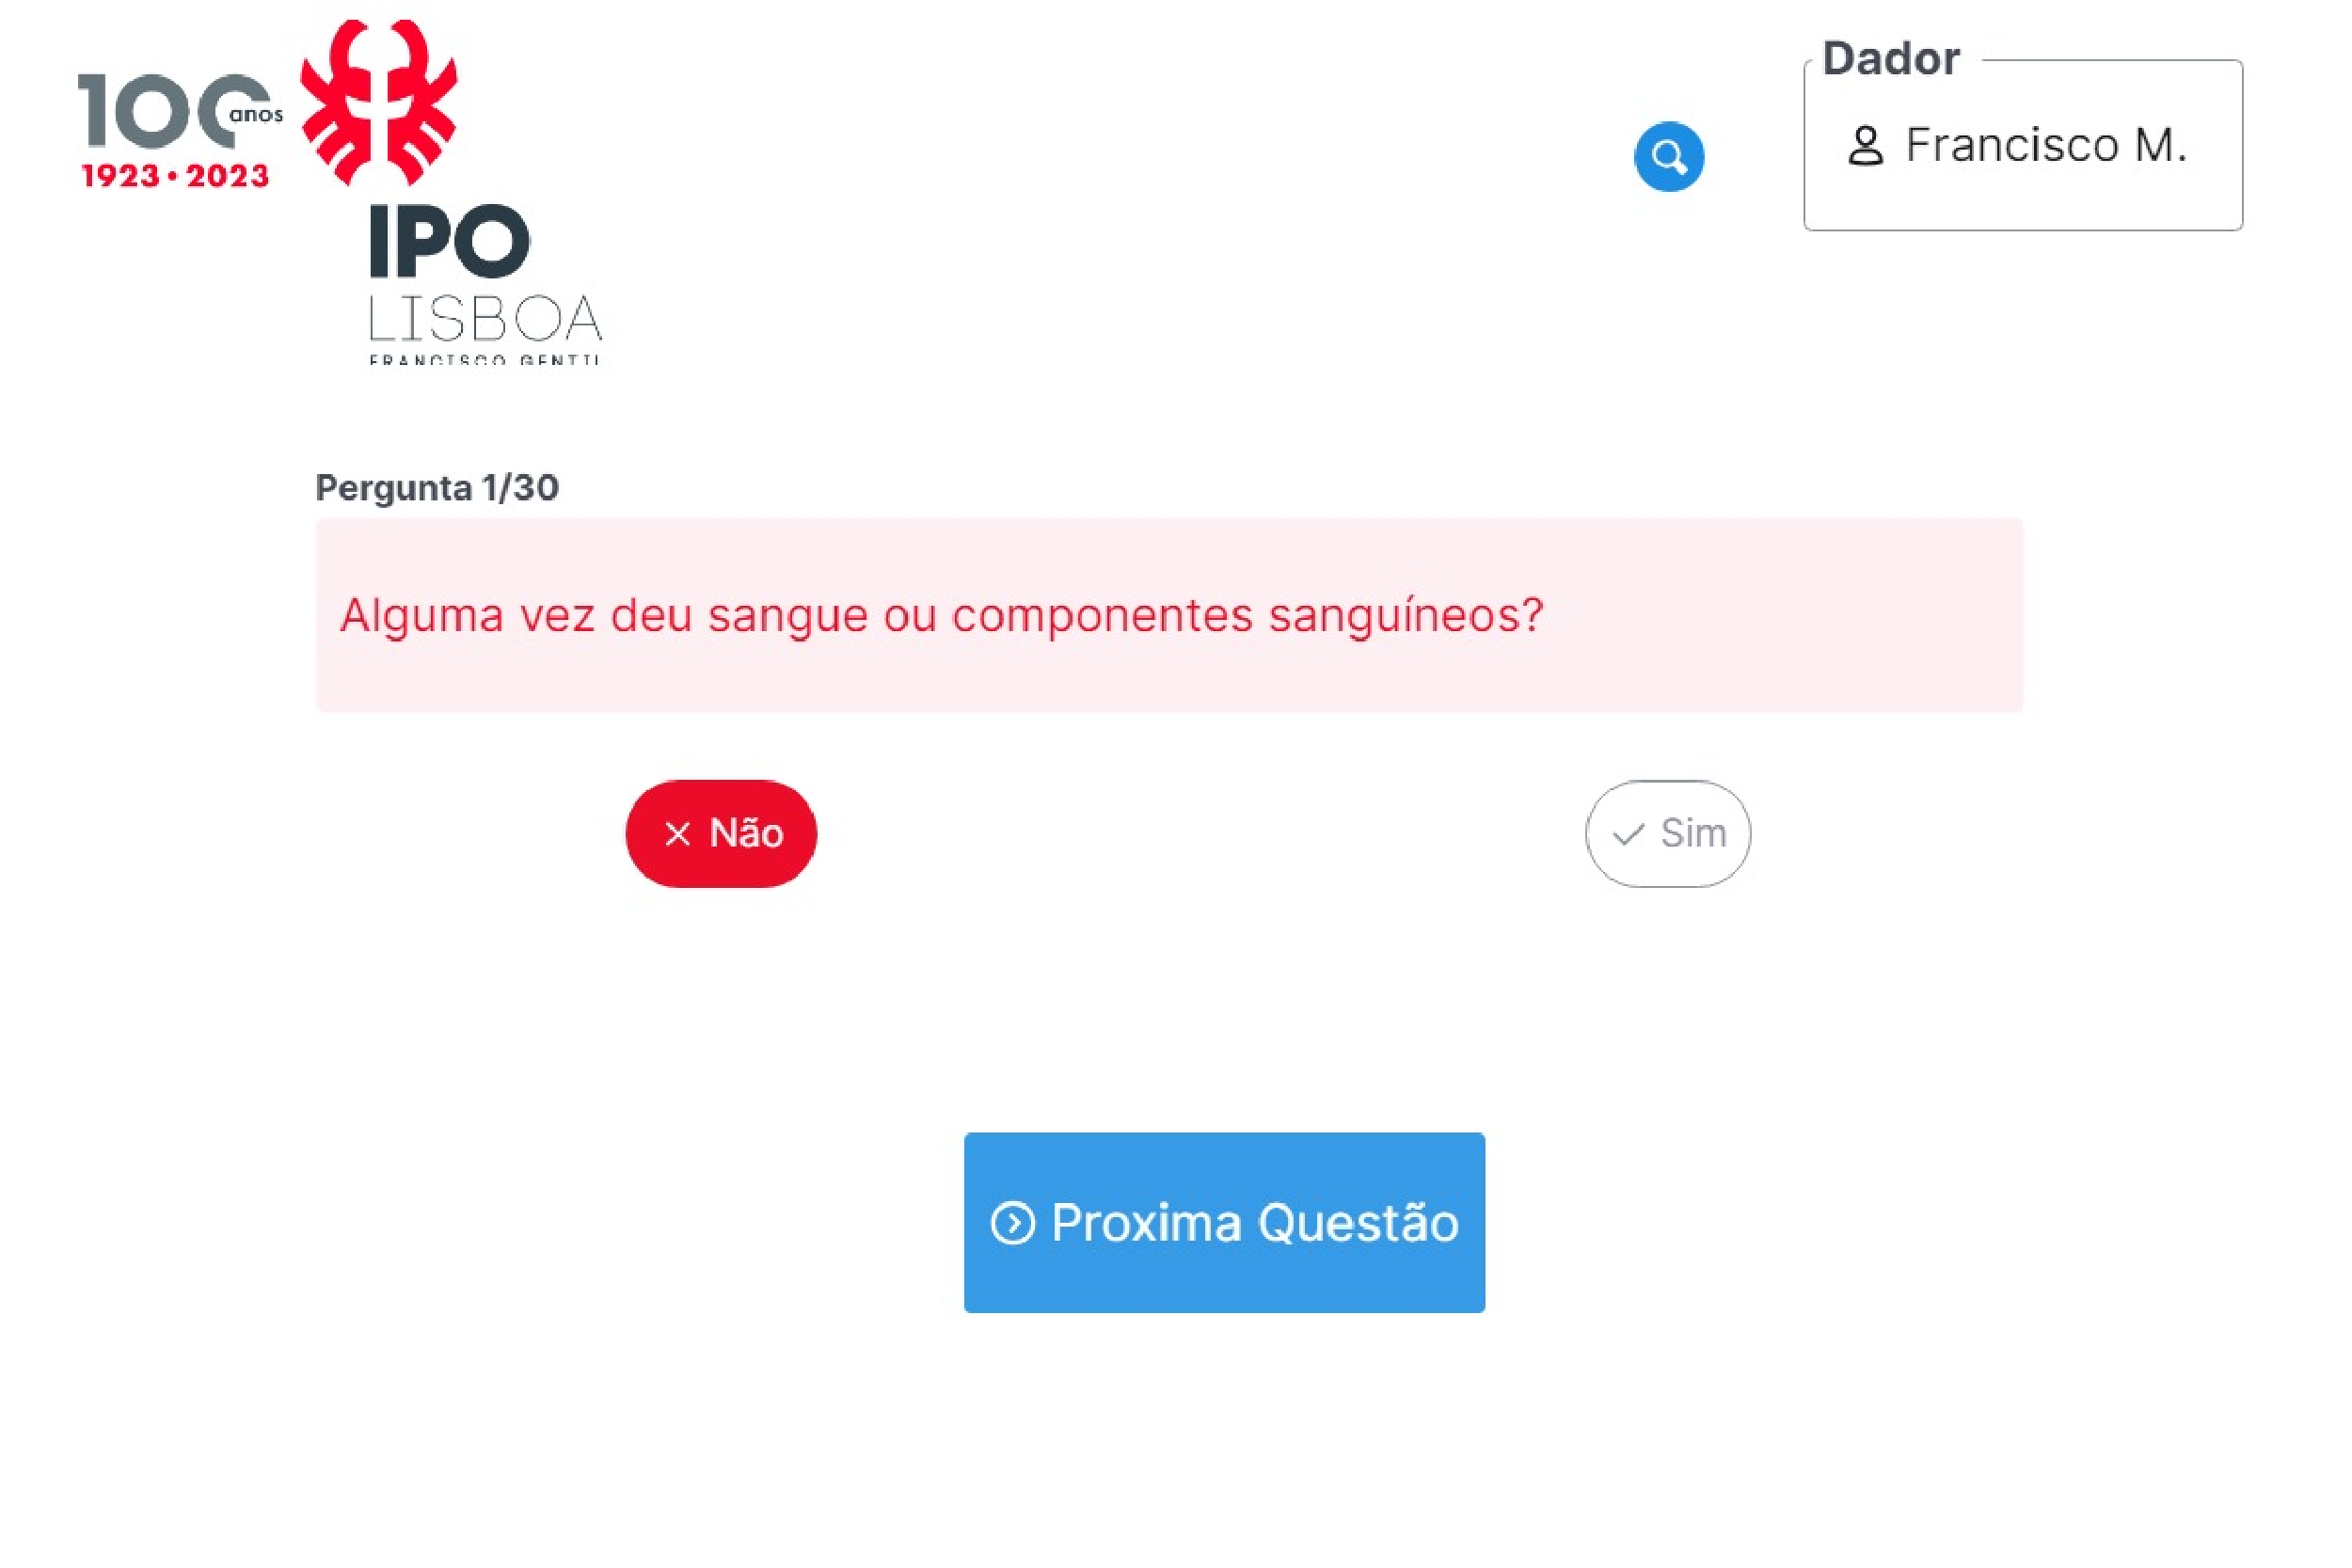
\includegraphics{./figures/Form_Answer_No.pdf}}
	\end{center}
	\caption{Form Page Negative Answer Mock.}\label{fig:form_no}
\end{figure}

\begin{figure}[H]
	\begin{center}
		\resizebox{160mm}{!}{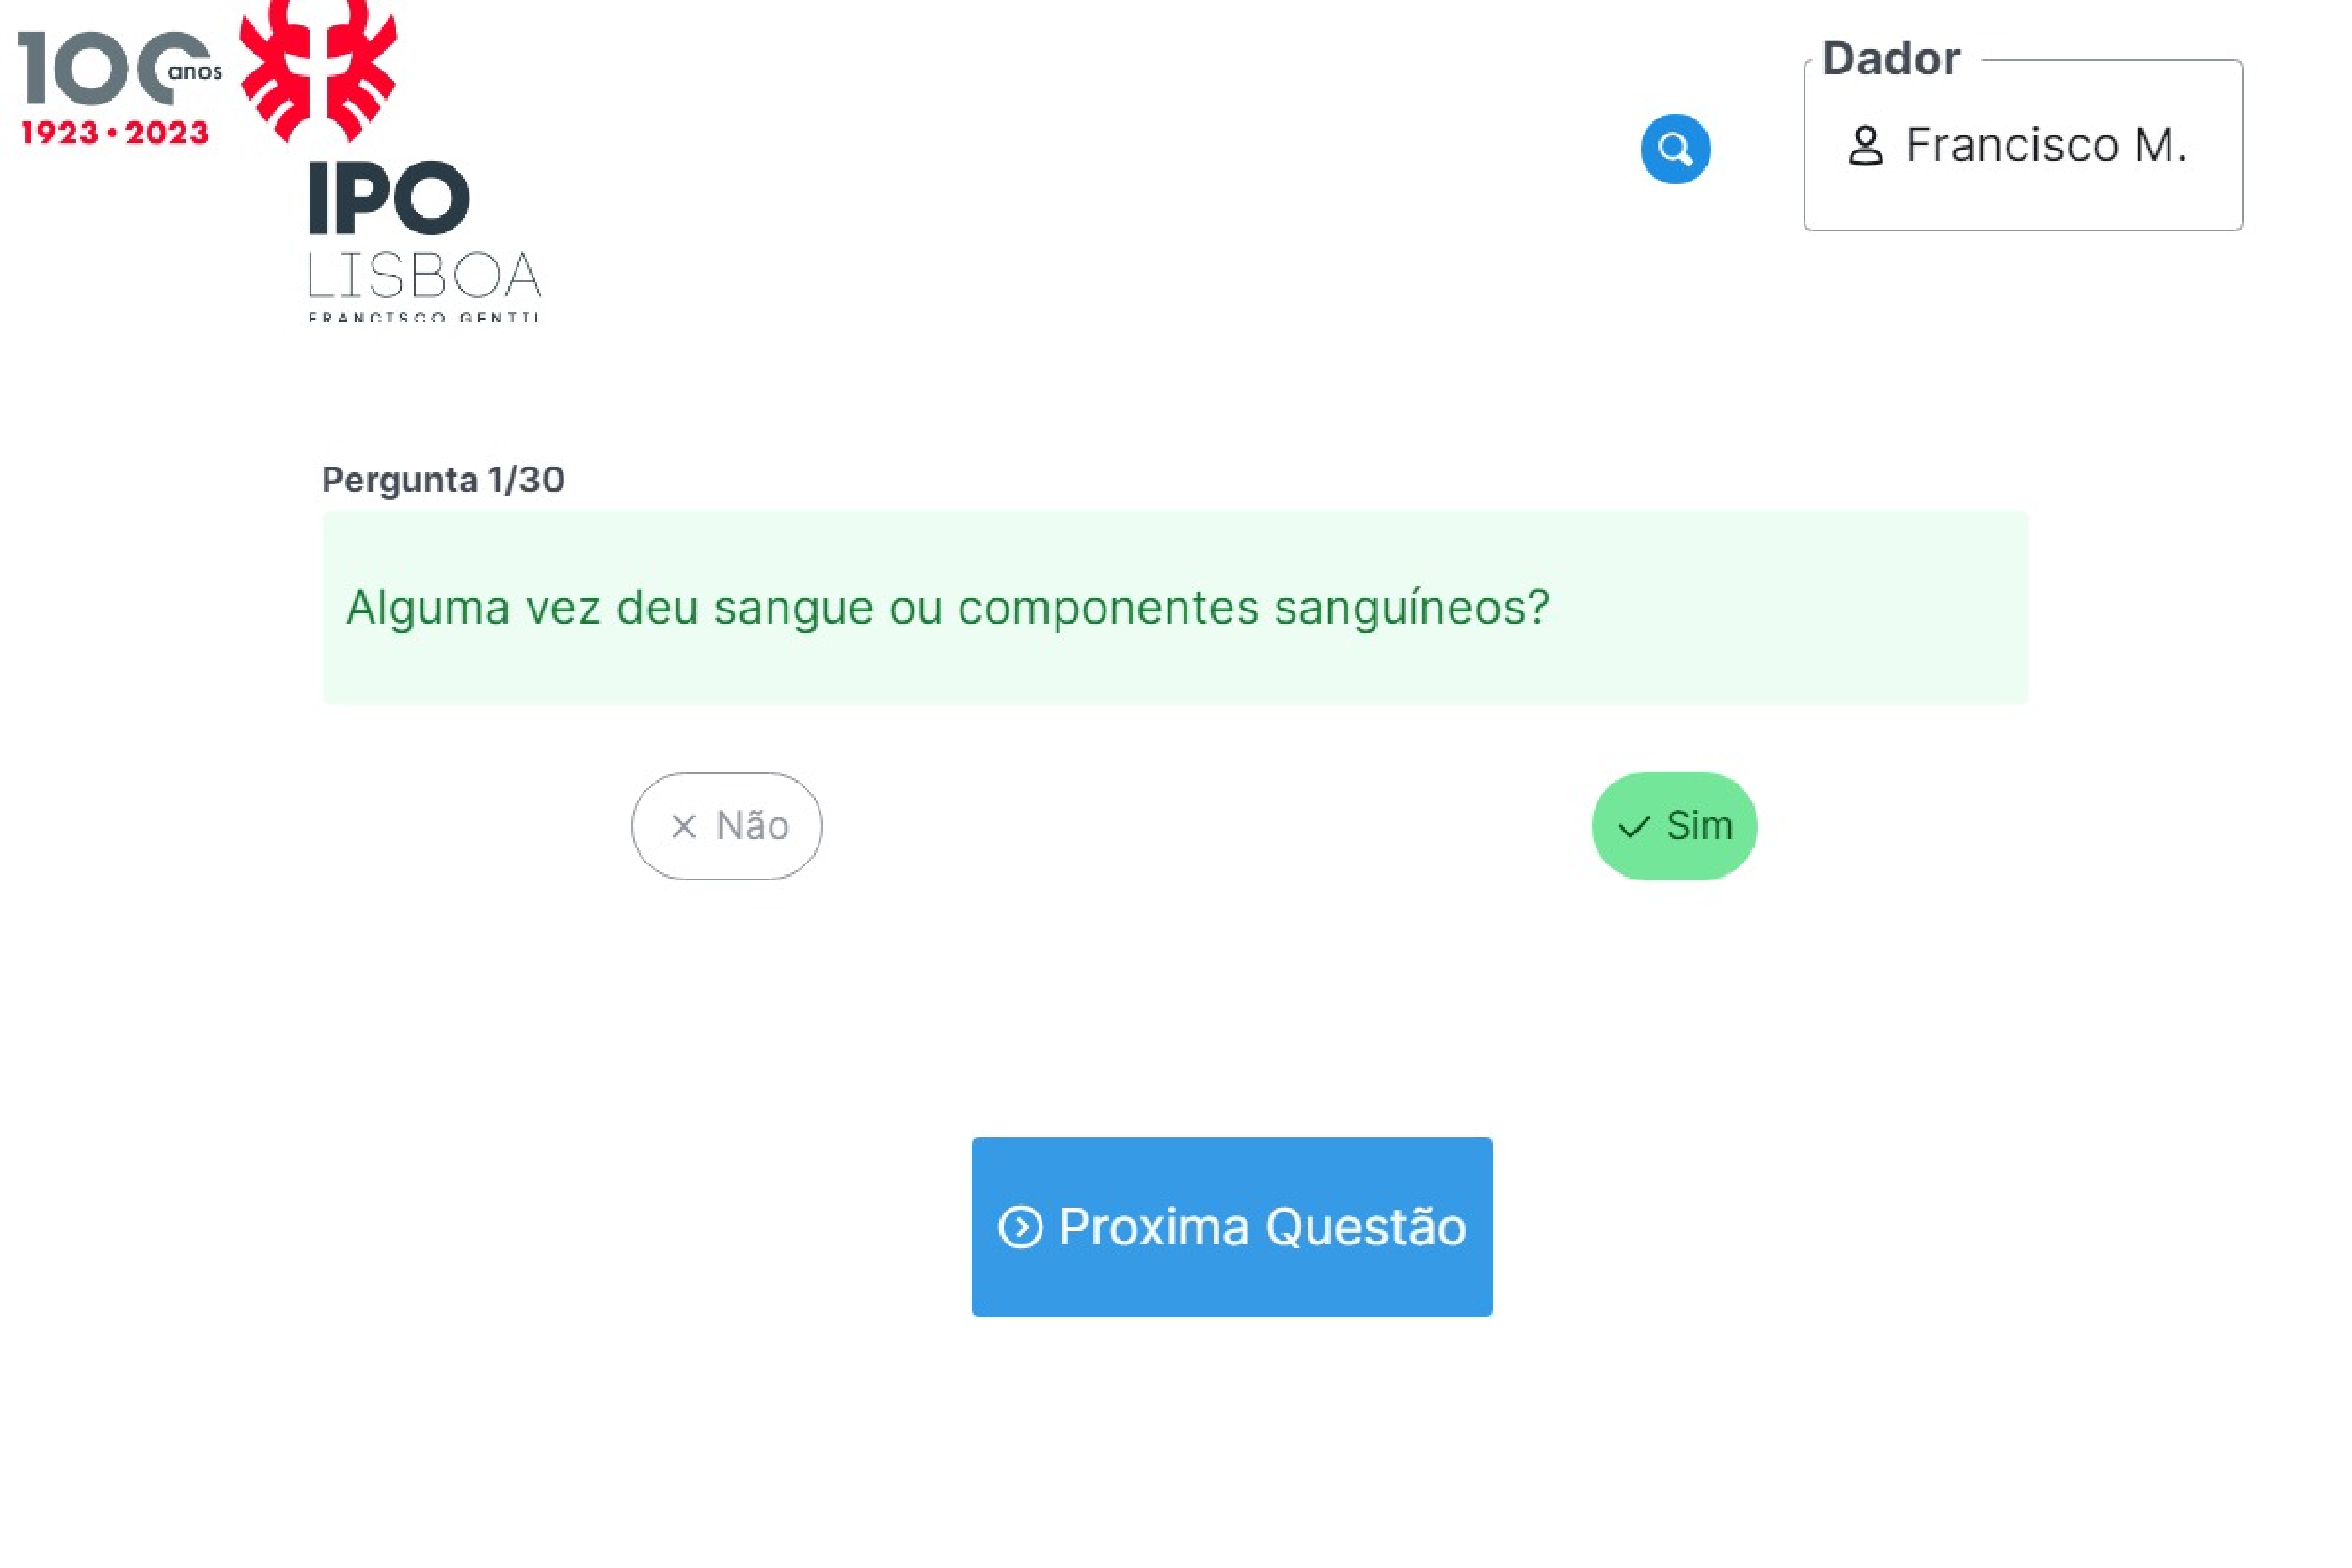
\includegraphics{./figures/Form_Answer_Yes.pdf}}
	\end{center}
	\caption{Form Page Positive Answer Mock.}\label{fig:form_yes}
\end{figure}

\begin{figure}[H]
	\begin{center}
		\resizebox{160mm}{!}{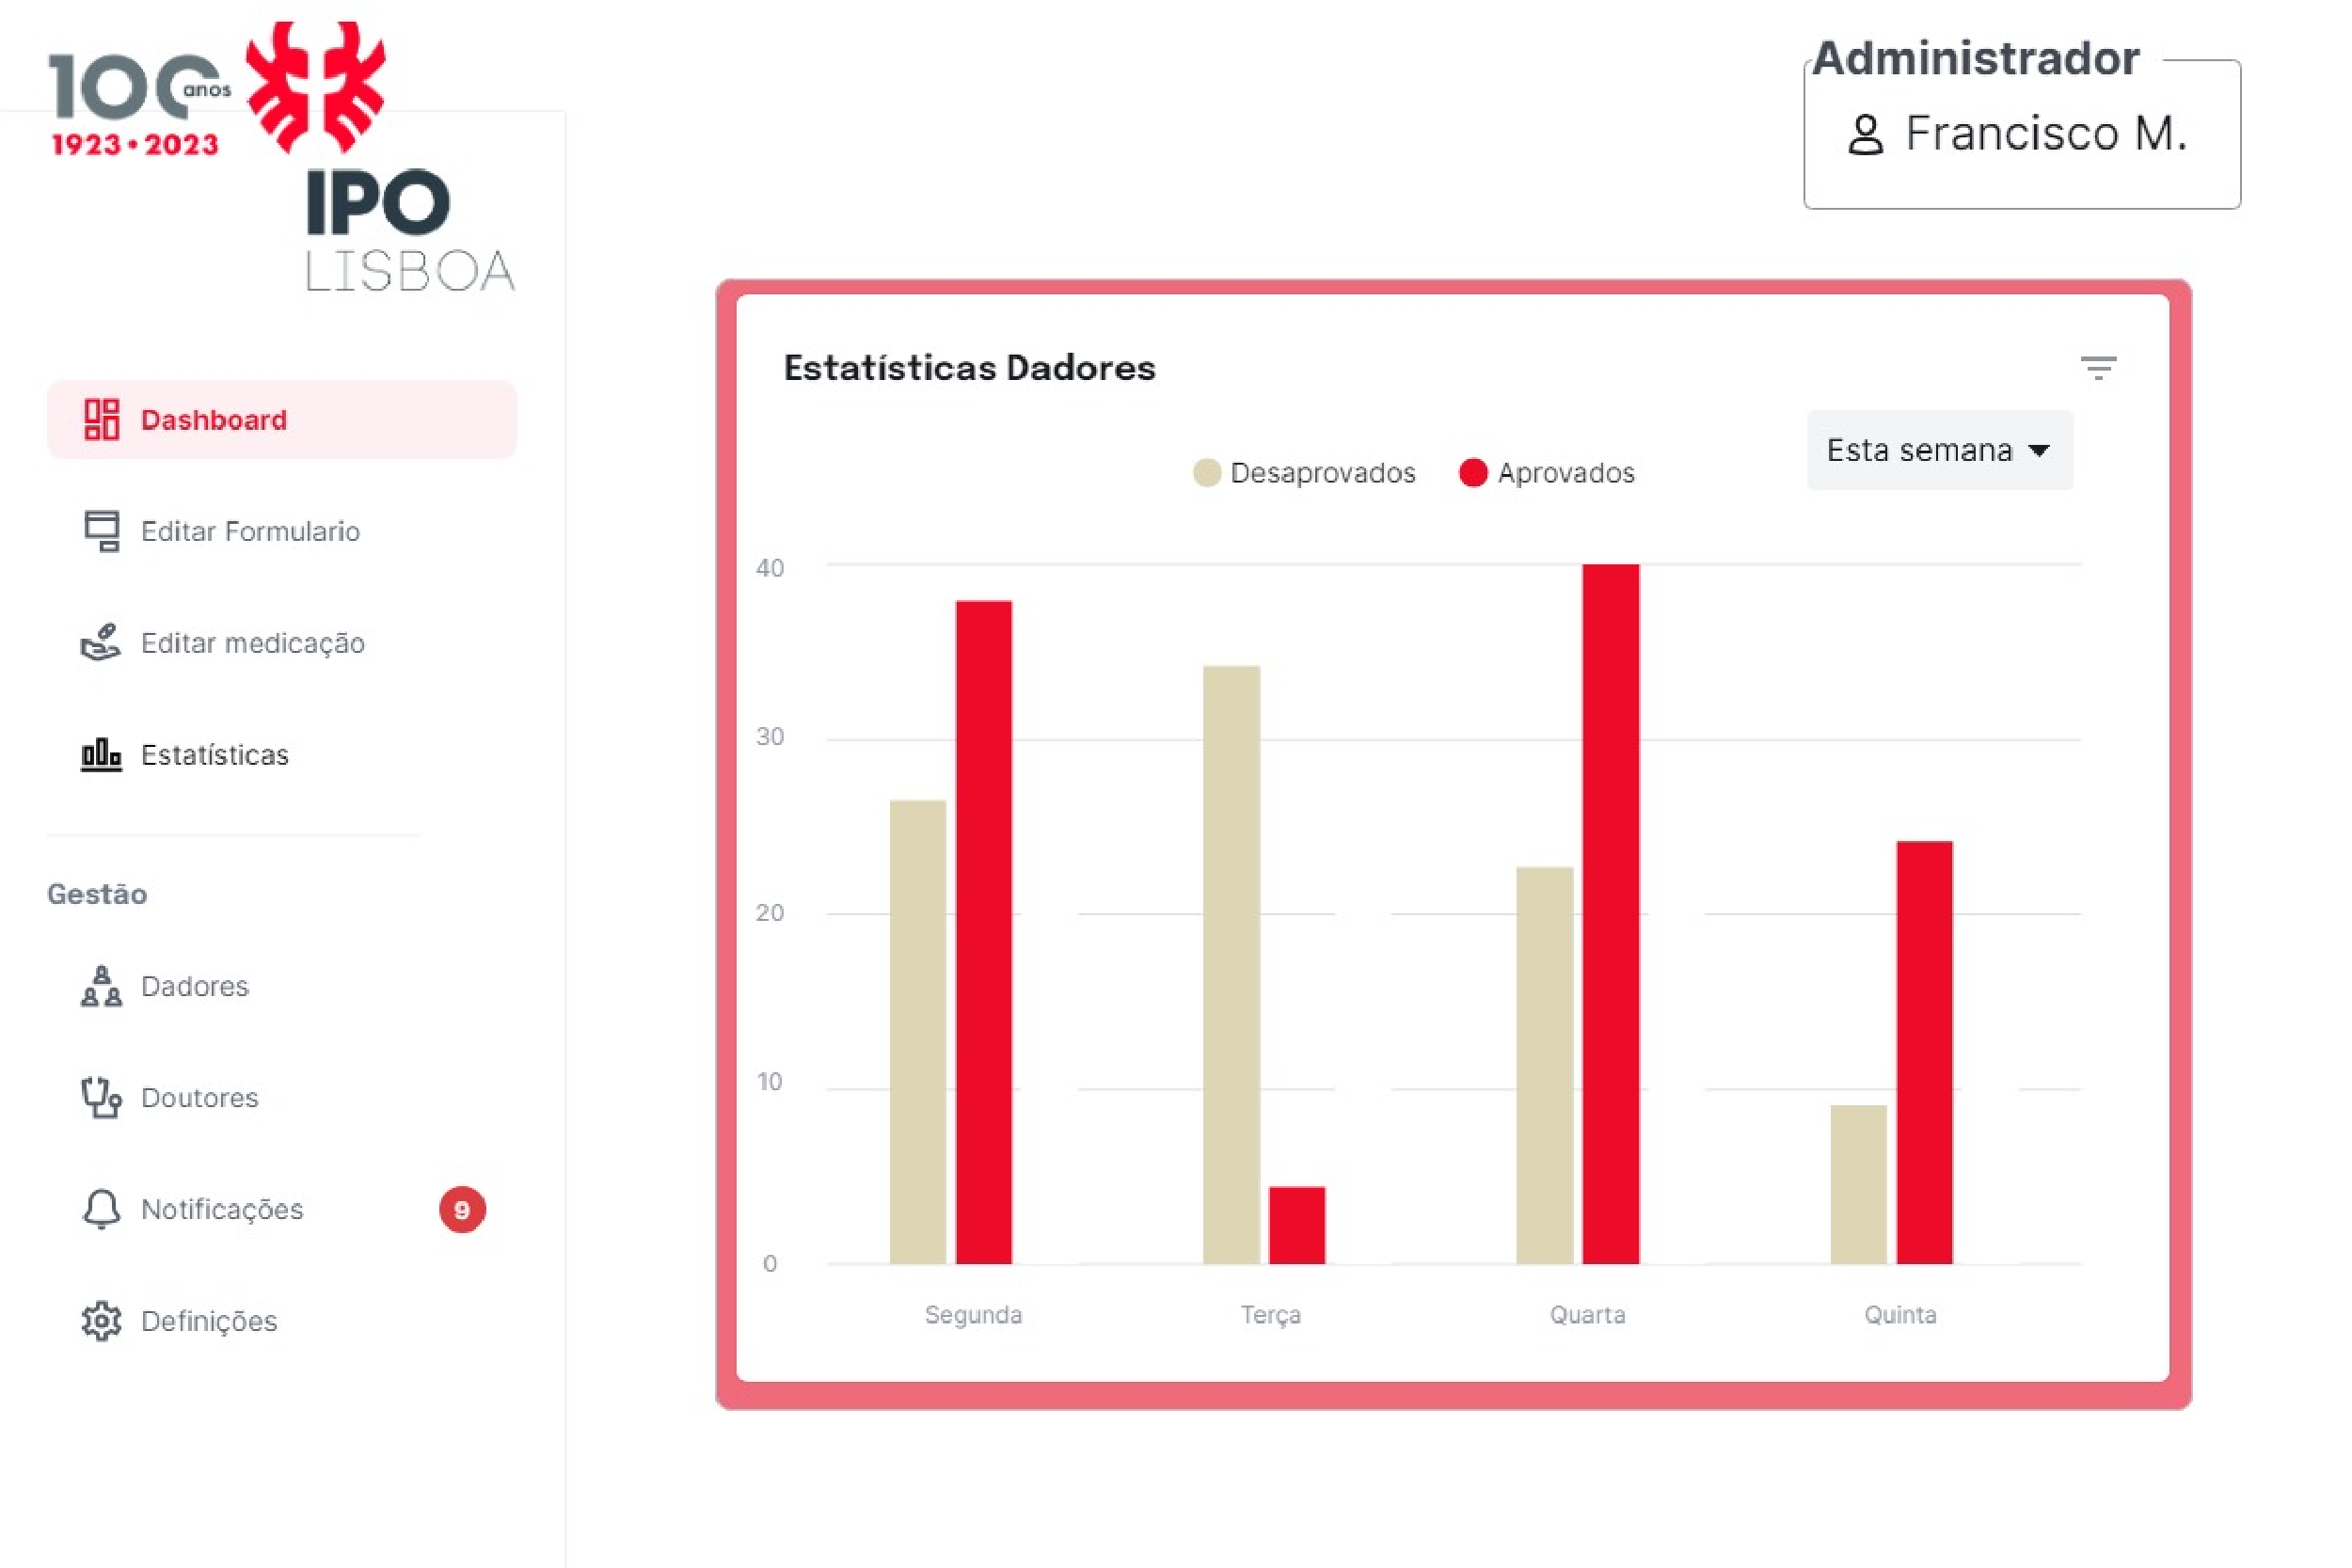
\includegraphics{./figures/Backoffice.pdf}}
	\end{center}
	\caption{Backoffice Page Mock.}\label{fig:backoffice}
\end{figure}




%\subsection{Form Services}
%
%The form service is responsible for managing the form resources.
%Figure ~\ref{fig:form_services} is a diagram that shows the architecture of the form services.
%
%\begin{figure}[htbp]
%	\begin{center}
%		\resizebox{150mm}{!}{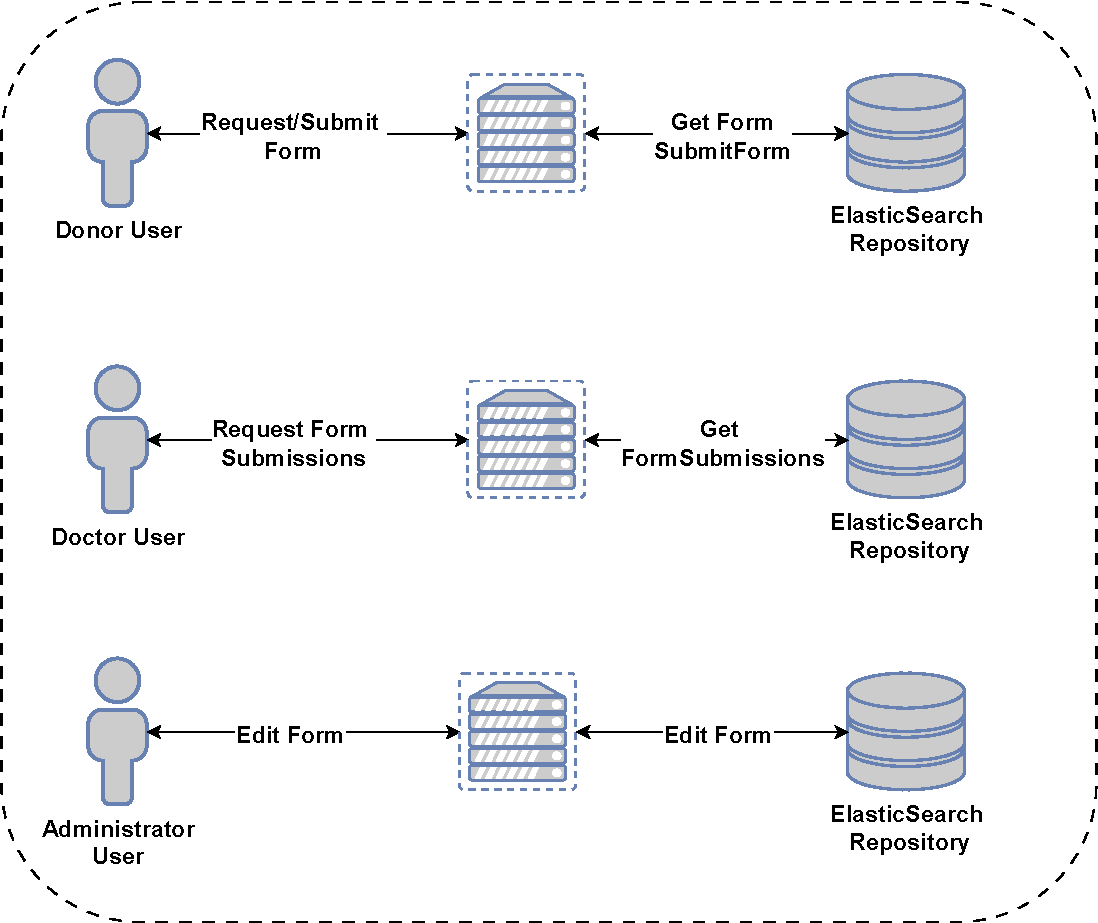
\includegraphics{./figures/formServices.pdf}}
%	\end{center}
%	\caption{Final Form Data Structure.}\label{fig:form_services}
%\end{figure}
